\blankpage
\thispagestyle{empty}
\vspace*{\fill}
\begin{center}

\includegraphics[width=5cm]{./imgs/bella.jpg}
\end{center}
\vspace*{\fill}

\pagestyle{plain}
\chapter{Sobre os autores}\label{part16}

\begingroup\small

\textbf{CATARINA II }\medskip

\noindent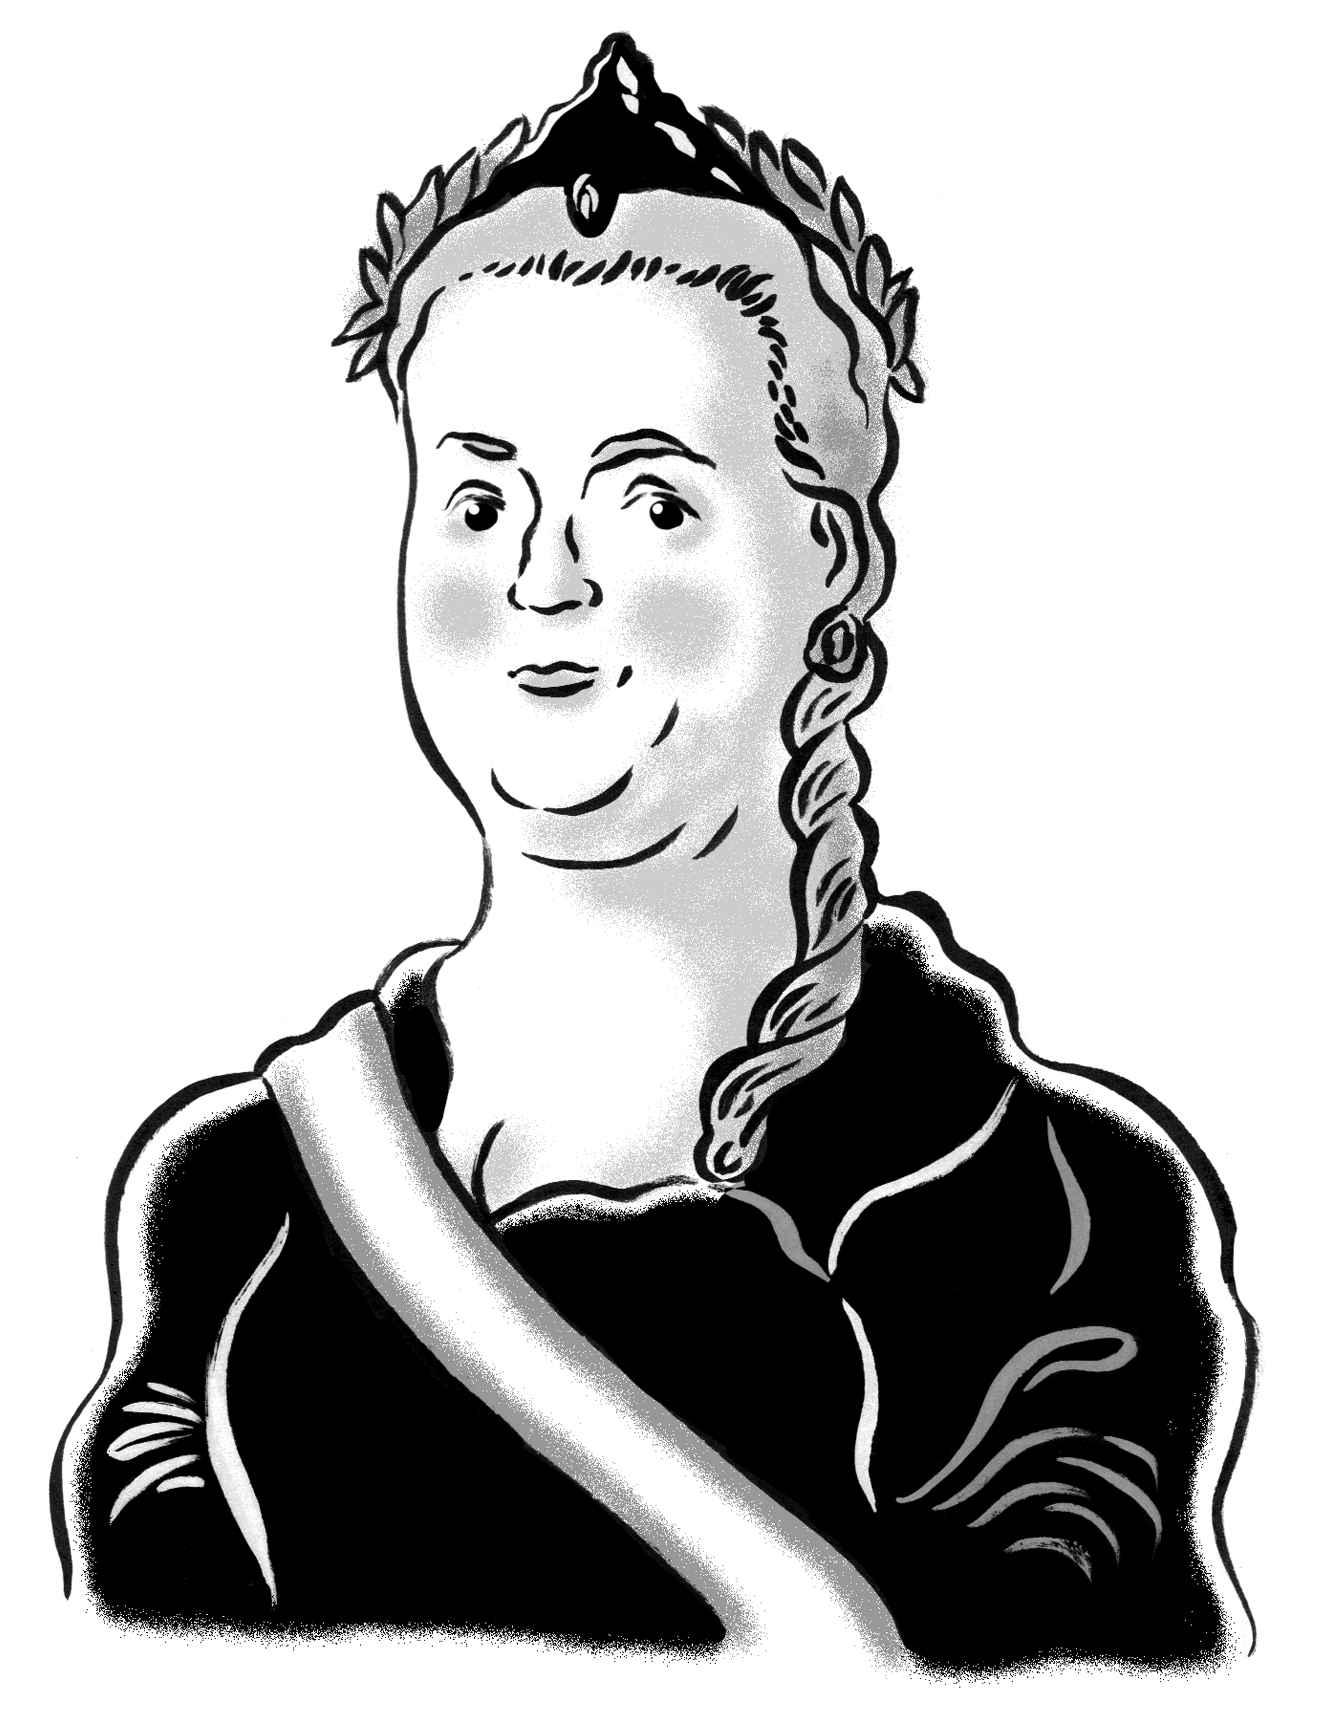
\includegraphics[width=.8in]{./imgs/autor1.jpg}

\noindent{}Os primeiros contos russos para infância saíram da pena de Catarina \textsc{ii}
(1729--1796), a imperatriz da Rússia de 1762 a 1796: ``Conto do
tsarévitche Cloro'' e ``Conto do tsarévitche Fevei'', duas parábolas universais.

Leitora aplicada, a própria tsarina, além de trocar correspondências com
pensadores célebres, aventurou"-se na escrita.

Catarina nasceu Sophie Friederike Auguste, na antiga Prússia, e, ao
casar"-se com o futuro Pedro \textsc{iii} e converter"-se à fé ortodoxa, adotou o nome
russo.

Nos 34 anos de seu governo, ela aprofundou o processo de ocidentalização
iniciado por Pedro, o Grande, e promoveu a ciência e as artes. Foi sua
coleção particular, incluindo 13 quadros de Rembrandt e 11 de Rubens,
que deu origem ao acervo do Museu Hermitage; em 1764, graças a seu
empenho, foi inaugurado o Instituto Smólny para moças nobres, a primeira
instituição educacional para mulheres da Rússia; também foram criados,
com seu incentivo, arquivos, tipografias, bibliotecas.

Mesmo com os avanços nas ciências e algumas ideias progressistas, seu
reino foi marcado pelos privilégios que cedera aos nobres e pela falta
de liberdade e de direitos dos camponeses, a maior parte da população.
Não por acaso Emelian Pugatchóv (c. 1742--1775) comandou um levante
camponês em 1773/1774, acontecimento descrito na novela \emph{A filha do
capitão} (1836), de Aleksándr Púchkin.


Catarina \textsc{ii} escreveu ``Conto do tsarévitche Cloro'' (\emph{Skazka o tsariévitche Khlore}) em 1781 para seus
netos Constantino e Alexandre, futuro imperador, e o texto tornou"-se um
dos mais conhecidos dela, sendo publicado em forma de livro em 1781,
1782 e 1783. Nesta última edição, a tiragem foi de 800 exemplares (400
em russo e 400 em grego).\footnote{\scriptsize\textsc{kravtchenko}, O. A. “Conto do tsarévitche Cloro” е o desenvolvimento do sistema alegórico e figurado na ode “Felícia” de G. R. Derjávin (\textit{“Skazka o tsariévitche Khlore” i púti razvitia eio óbrazno-allegorítcheskogo stroia v ode G. R. Derjávina “Felitsa”}). \textit{Imalologuia i komparativistka}, 2015, nº1, pp. 91–104.p.\,91.} De teor iluminista e
universal, a obra utiliza em sua composição elementos de contos
populares ou folclóricos. Traduzido a partir dos
manuscritos disponíveis no site da Biblioteca Estatal Infantil da Rússia
(\textsc{rgdb}, Moscou).

\bigskip
\noindent\textbf{VLADÍMIR ODÓIEVSKI}\medskip

\noindent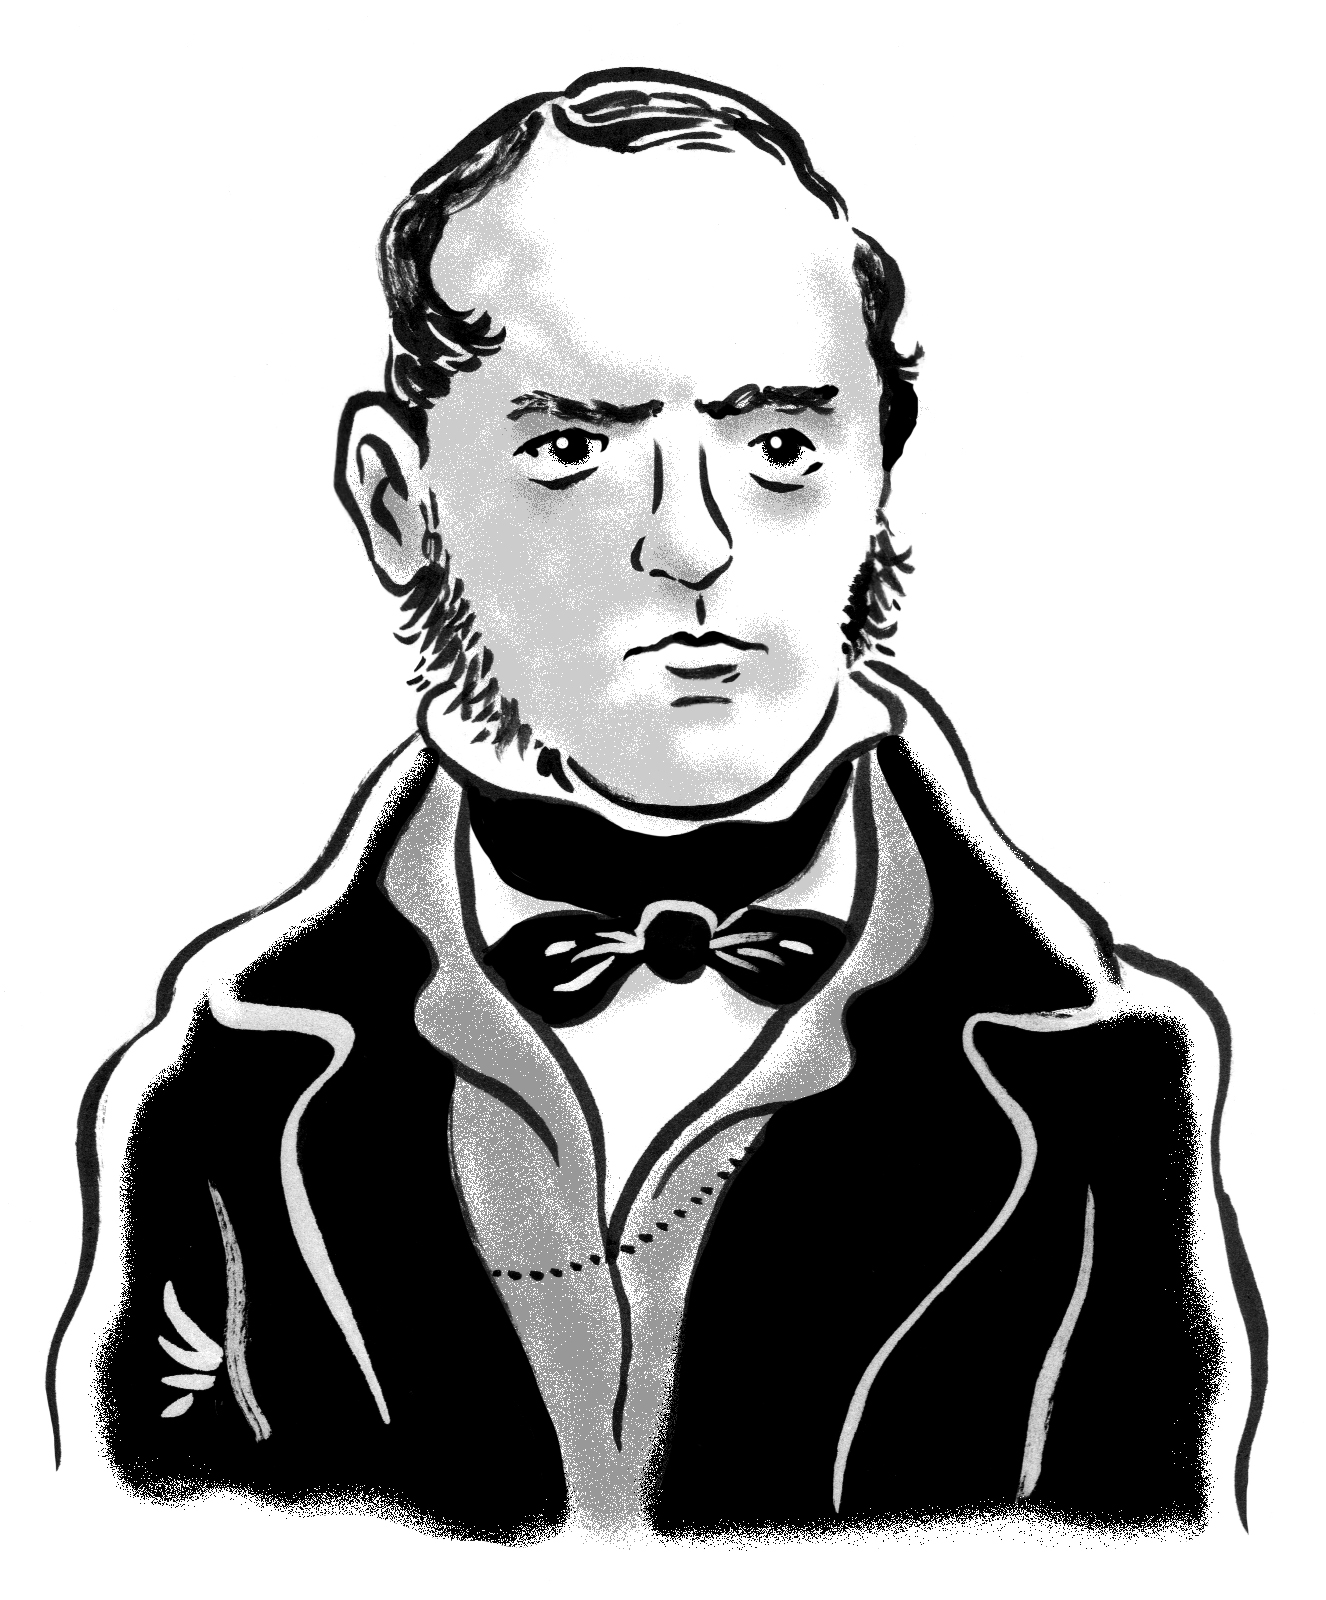
\includegraphics[width=.8in]{./imgs/autor2.jpg}

\noindent{}O príncipe Vladímir Odóievski (1804--1869) era musicólogo, escritor e
ocultista. Foi representante do romantismo russo, com influências de
Hoffman, Schelling (a quem conheceu pessoalmente) e do idealismo alemão.
Odóievski publicou em 1844 \emph{Noites russas,} romance de traços
românticos e filosóficos.

Como músico e musicólogo, acreditava que a ``música era filha da
matemática'', admirava Bach, Beethoven e Glinka, compôs músicas sobre
poemas de Púchkin e Nekrássov e para fábulas de Krylóv, foi autor dos
livros \emph{Alfabeto musical para escolas populares} e \emph{Gramática
musical para não músicos.}

Participava ativamente da vida literária, era amigo de Gógol e
Lêrmontov, e sua obra interessou a Púchkin, de quem foi ajudante na
revista que o poeta havia fundado, \emph{O contemporâneo.} Foi
Odóievski, por sinal, o autor da frase ``o sol da poesia russa'',
referindo"-se a Aleksándr Púchkin, que é repetida aos quatros ventos na
Rússia.

O príncipe também se interessou pela educação; ele acreditava que as
crianças deveriam desenvolver qualidades humanitárias e valorizar o
saber por um processo de aprendizagem não desquitado da realidade e
concebido como um todo, e não como um conjunto de disciplinas isoladas e
artificiais.\footnote{\scriptsize\textsc{sigóv}, Vladímir (org.). \textit{Literatura infantil} (\textit{Diétskaia literatura}). Moscou: Iurait, 2019, p. 83.}

Vladímir Odóievski começou a escrever textos para a infância nos anos
1830, com o pseudônimo ``titio Irinei'', e passou por vários gêneros.

``A cidadezinha da tabaqueira'' (\emph{Gorodók v tabakierke}), de traços
românticos, um marco das letras russas infantis, foi publicado em 1834
de forma independente, sendo depois integrado à coletânea \emph{Contos
do titio Irinei,} de 1841. O conto de Odóievski foi muito elogiado por
Belínski, que notou na caixinha de música em que Micha se
aventura uma alegoria da sociedade. Em 1976, Valéri Ugárov fez uma
animação psicodélica baseada no conto. Traduzido a partir de:
\textsc{odoiévski}, V. \emph{Pióstrye skasky. Skázki diéduchki Irineia.} Moscou:
\emph{Khudójestvennaia literatura,} 1993, pp.\,126--135.

\pagebreak
\noindent\textbf{IVAN TURGUÊNIEV}\medskip

\noindent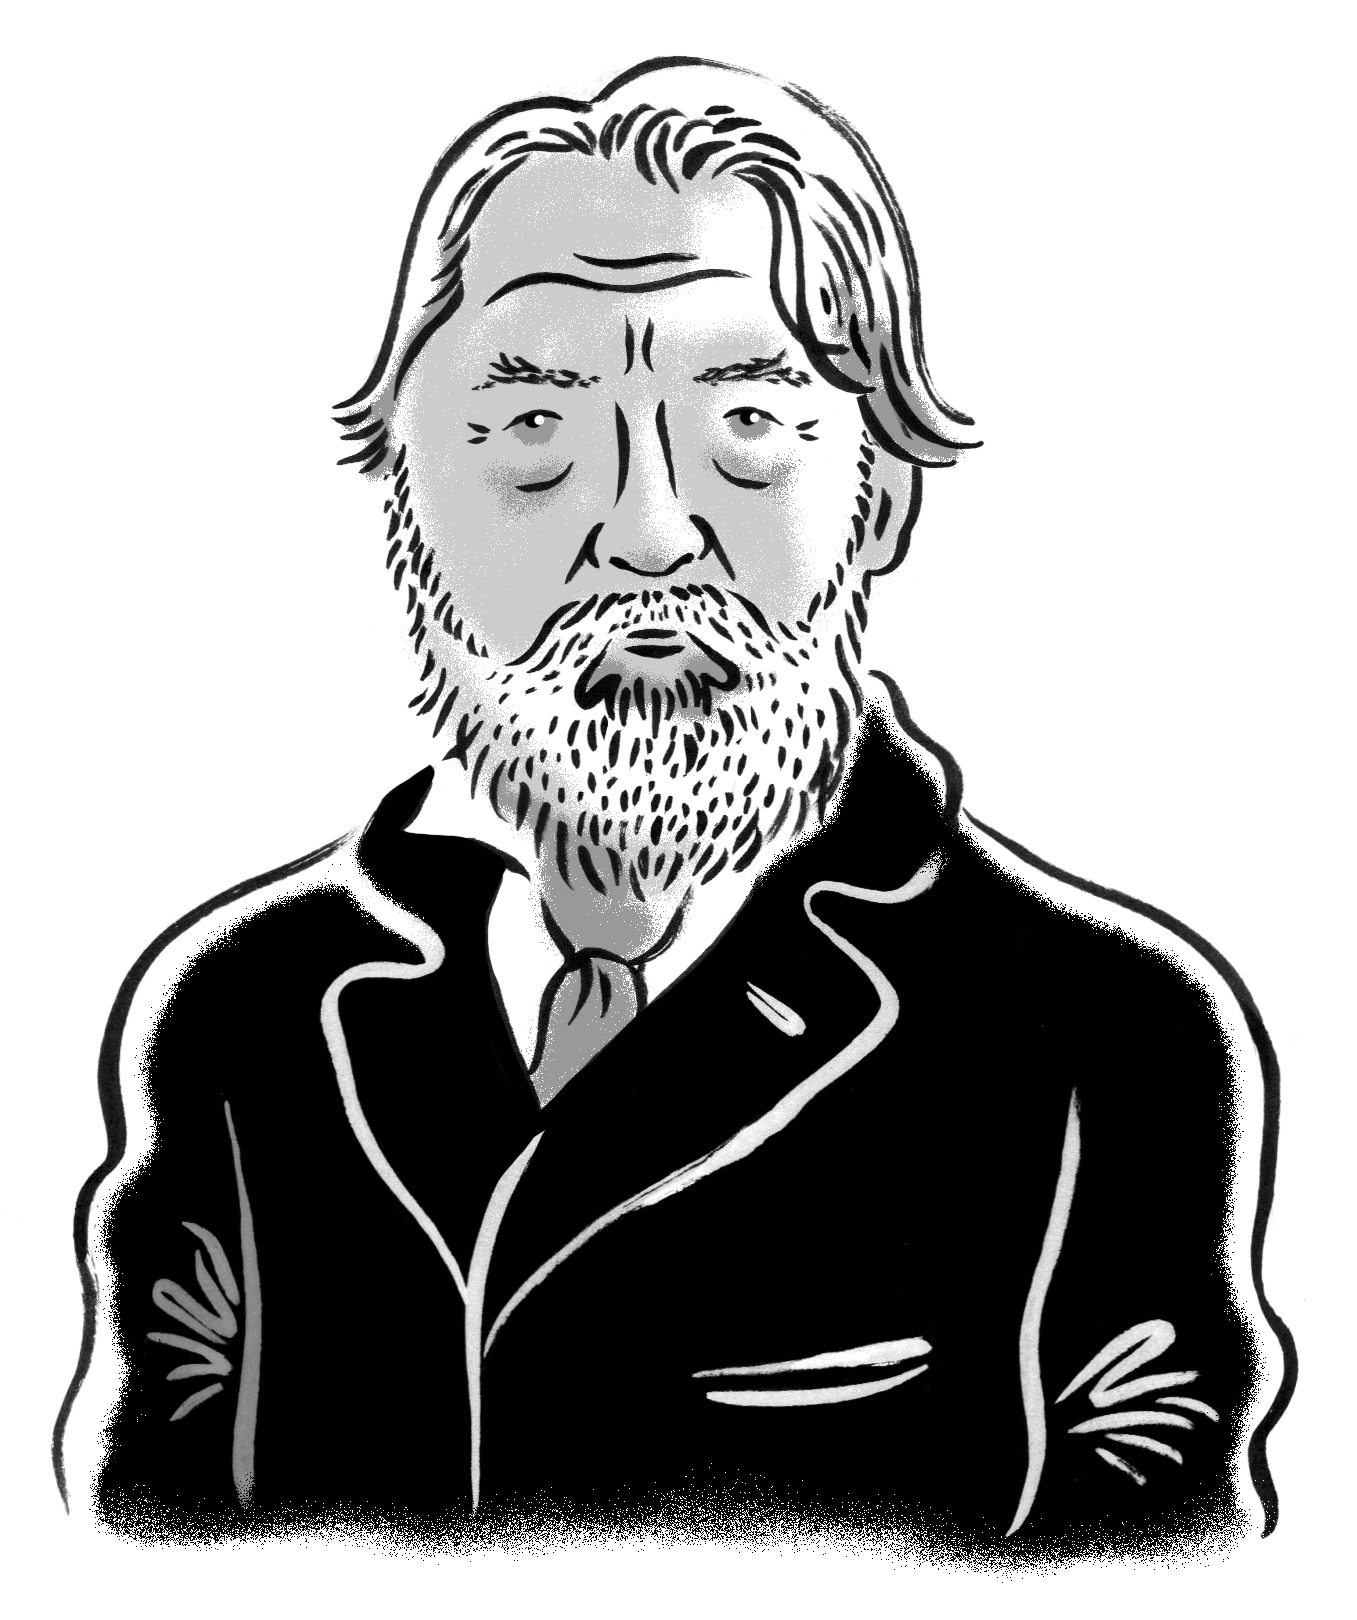
\includegraphics[width=.8in]{./imgs/autor3.jpg}

\noindent{}Quando se pensa em literatura russa, Ivan Turguêniev (1818--1883) é
daqueles autores inescapáveis. Suas obras, escritas com primor,
tornaram"-se conhecidas no mundo inteiro, tal como \emph{Pais e filhos}
(1862), dedicado ao crítico Vissarion Belínski.

De uma família nobre abastada, Turguêniev passou anos de sua vida na
Europa, mas nunca deixou de se sensibilizar com as questões da Rússia. O
interesse pelas transformações político"-sociais de seu país não o
impediu, no entanto, de expor em seus livros, que oscilavam entre
romantismo e realismo, grandes contradições humanas.

Nascido numa propriedade rural na região de Oriol, tinha um pai ausente,
que morreu aos 42 anos, e uma mãe voluntariosa e autoritária, Varvara
Turguênieva. Em 1833, o futuro escritor ingressou no
departamento de letras da Universidade de Moscou e, um ano depois,
transferiu"-se para a Universidade de São Petersburgo, onde se graduou em
1837, partindo para Berlim para continuar os estudos. A Alemanha foi
também palco do encontro que teve com Mikhail Bakúnin, no começo da
década de 1840, figura que em parte inspirou seu primeiro
romance, \emph{Rúdin}, de 1856.

A vida de Ivan Turguêniev sofreu uma guinada em 1843, quando ele
conheceu em São Petersburgo a cantora lírica e compositora francesa
Pauline Viardot e por ela se apaixonou perdidamente. Era casada com o
crítico e diretor de teatro Louis Viardot, vinte anos mais velho que
ela, mas isso não conteve Turguêniev, que não mais se afastou de sua
amada. A devoção dele por Pauline motivou nova temporada na Europa, onde
ele manteve contato com grandes nomes das letras francesas, como George
Sand, Gustave Flaubert e Victor Hugo.

Desde os anos 1830, o jovem Turguêniev, fanático por Púchkin e Gógol, já traduzia e
escrevia poemas e peças, mas sua entrada definitiva para o mundo
literário se deu em 1847, quando começou a publicar, na revista \emph{O
contemporâneo,} os contos que formariam o volume de \emph{Memórias de um
caçador} (1852), coletânea que colaborou para o fim do regime de
servidão da gleba. A partir de então escreveu principalmente
textos em prosa, muitos dos quais se tornaram clássicos, tais como:
\emph{Diário de um homem supérfluo} (1850), \emph{Ássia} (1858), \emph{Primeiro amor} (1860).

Iván Turguêniev morreu em 1883 em Paris, mas pediu que fosse enterrado
em São Petersburgo.

\textls[-10]{``Mumu'' saiu pela primeira vez na revista \emph{O contemporâneo}, em
1854, mas foi escrito antes, em 1852, na época em que Turguêniev cumpria
prisão domiciliar de 18 meses, após ter publicado um necrológio de
Nikolai Gógol. Ao aparecer na revista, o texto foi considerado
``impróprio para publicação'' e só pôde ser integrado às obras completas
do autor em 1856. Muito popular na Rússia, a história de Guerássim
comove gerações de leitores, que se questionam por que ele sacrificou a
única criatura que amava. Sabe"-se também que a personagem foi baseada em
um criado da mãe de Turguêniev, o mudo Andrei, que afogou sua
cachorrinha Mumu a mando da patroa, mas, ao contrário de Guerássim, aquele
continuou trabalhando com ela.\footnote{\scriptsize\textsc{darmaros}, Marina. \emph{Material digital
  do professor} --- \emph{Contos russos juvenis.} São Paulo: Kalinka, 2021.}
Traduzido a partir de:
\textsc{turguêniev}, I. \emph{Pólnoie sobránie sotchiniénii i pissem v 30
tomákh.} Moscou: \emph{Naúka,} 1980.}

\bigskip
\noindent\textbf{LEV TOLSTÓI}\medskip

\noindent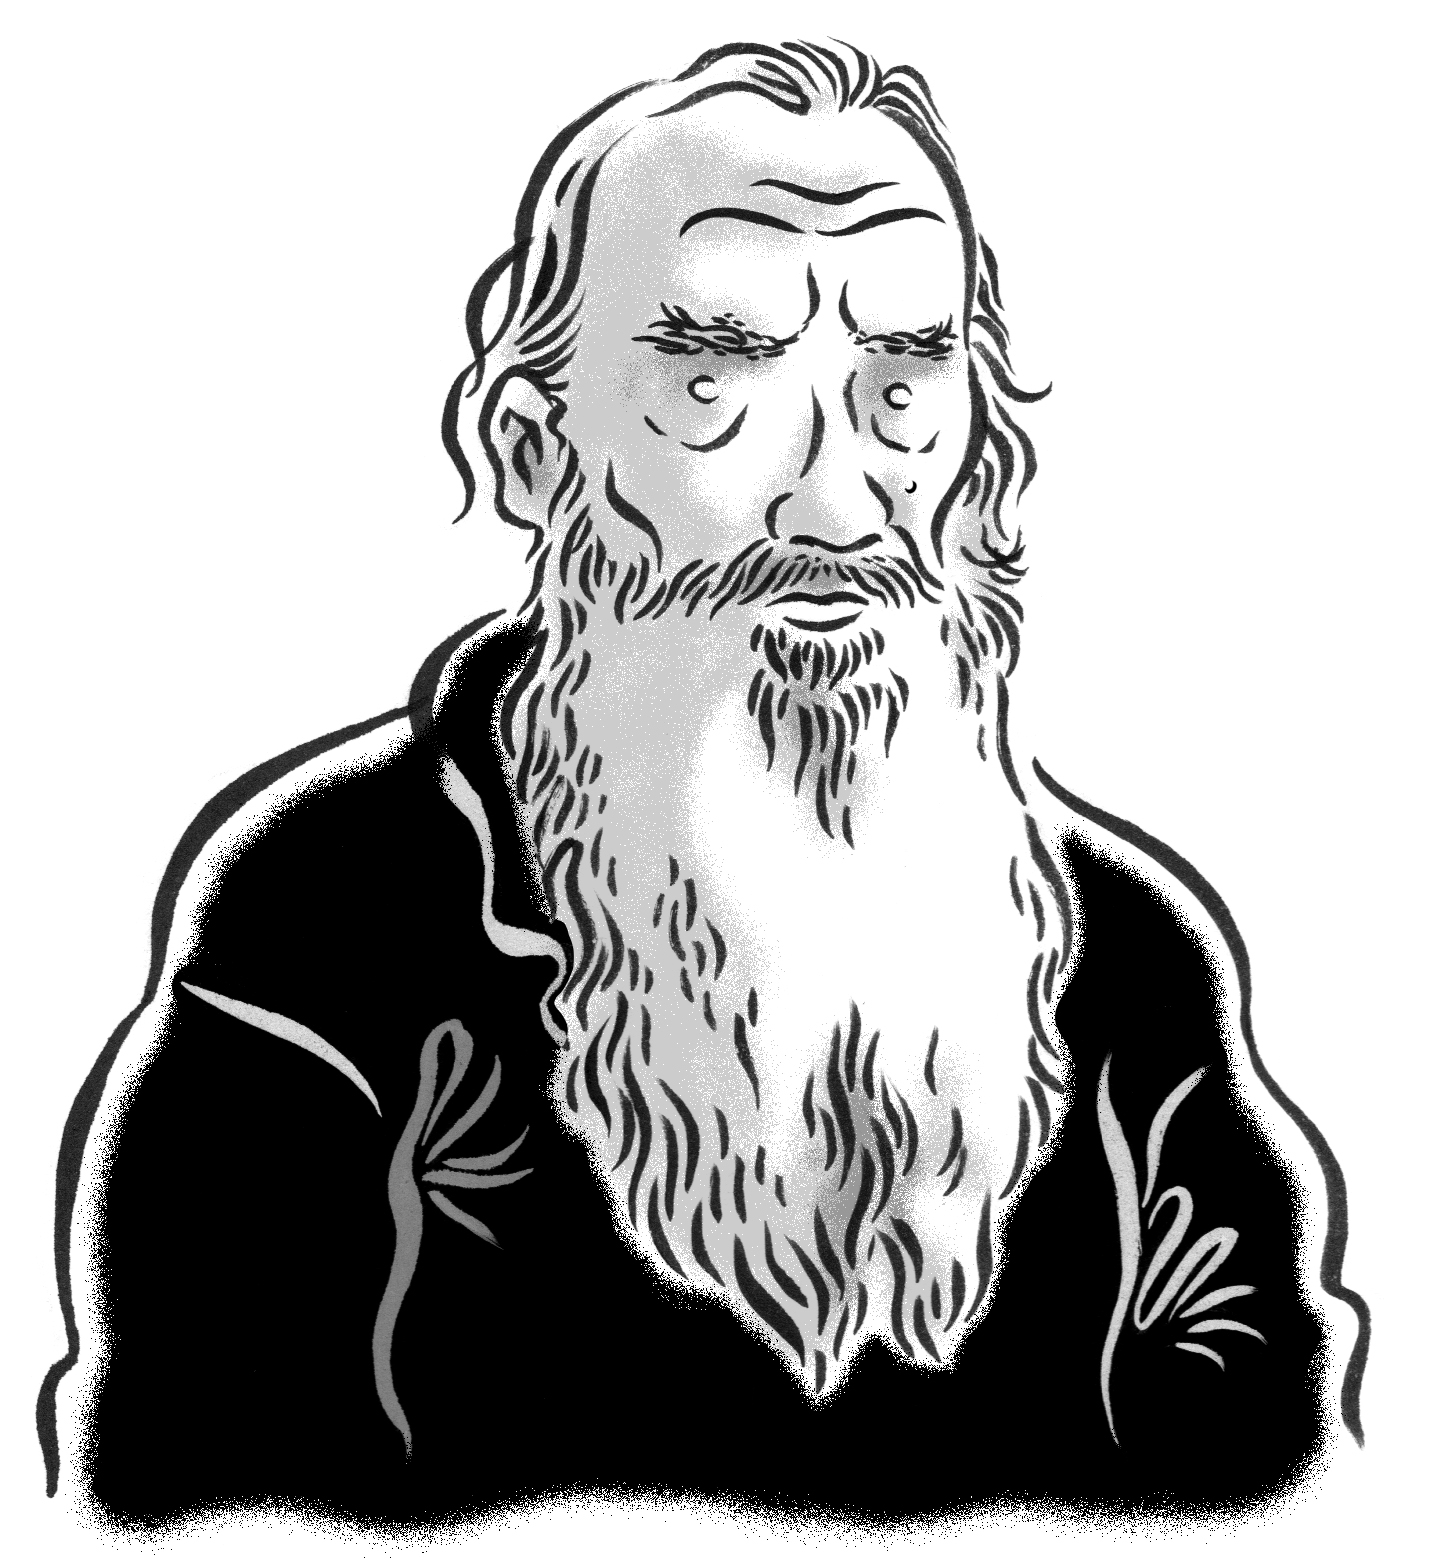
\includegraphics[width=.8in]{./imgs/autor4.jpg}

\noindent{}Nem todo mundo sabe que o conde Lev Tolstói (1828--1910) dedicou
praticamente toda a sua vida também à educação e à literatura para a
infância e a juventude. Além de ter fundado, em 1859, uma escola para
camponeses na propriedade onde nascera, Iásnaia Poliana, ele criou a
\emph{Cartilha} (1871--1872), enorme manual depois desmembrado na
\emph{Nova cartilha} (1875) e em quatro \emph{Livros russos para
leitura} (1875--1885).

Tendo perdido os pais ainda menino, Tolstói foi educado por tutores e
depois por uma tia. Ele ingressou, em 1845, na Universidade de Kazan,
mas não chegou a concluí"-la, sendo, no fim das contas, um autodidata ---
era conhecedor de muitas línguas e filosofias.

Foi durante o serviço militar, passando pelo Cáucaso e pela Crimeia, que
começou a escrever. Seu primeiro texto, \emph{Infância,} saiu em 1852 na
revista \emph{O contemporâneo.} A fase de seus longos romances, de
\emph{Guerra e paz} (1865--69) até \emph{Anna Kariénina} (1875--77),
começou após seu casamento, em 1862, com Sófia Andréievna, união que
gerou 13 filhos.

Tomado por anseios e inquietações, o escritor intercalou vida literária
e outros interesses. ``Tolstói é importante não apenas por ser o mestre
insuperado do gênero que se costumou chamar `romance psicológico do
século \textsc{xix}', mas também por seus contos breves, diários e escritos
teóricos sobre pedagogia, arte e religião''.\footnote{\scriptsize\textsc{bernardini}, Aurora Fornoni. \textit{Aulas de literatura russa: de Púchkin a Gorenstein}. São Paulo, Kalinka, 2018.p.\,138.}

A década de 1880 aprofundou uma série de crises existenciais por que o
escritor havia passado e o levou a uma fase que ele próprio definiu como
sua ``redenção moral''. Já praticante do vegetarianismo, ele abriu mão
dos direitos autorais de algumas obras em prol dos camponeses e
sistematizou uma série de preceitos filosóficos e religiosos que,
reunidos, passaram a ser conhecidos como \emph{tolstoísmo}, doutrina
baseada no cristianismo, mas acrescida de outras concepções, que
repercutiu no mundo todo e fez com que Tolstói fosse excomungado da
Igreja Ortodoxa. Seu último romance foi \emph{Ressurreição} (1899).

``O prisioneiro do Cáucaso'' (\emph{Kаvkázskii pliénnik}), que trata do
conflito clássico entre russos e tchetchenos ou entre colonizados e
colonizadores, foi escrito por Tolstói para ser incluído no quarto \emph{Livro russo
para leitura} e também foi publicado na revista \emph{Aurora}
(\emph{Zariá}) em 1872. A história, muito conhecida dos russos,
foi adaptada duas vezes para o cinema.
Traduzido a partir de:
\textsc{tolstói}, L. \emph{Sobránie sotchiniénii v 22 tt}. Moscou:
\emph{Khudójestvennaia literatura}, 1982, tomo 10, pp.\,208--230.

\bigskip
\noindent\textbf{NIKOLAI LESKÓV}\medskip

\noindent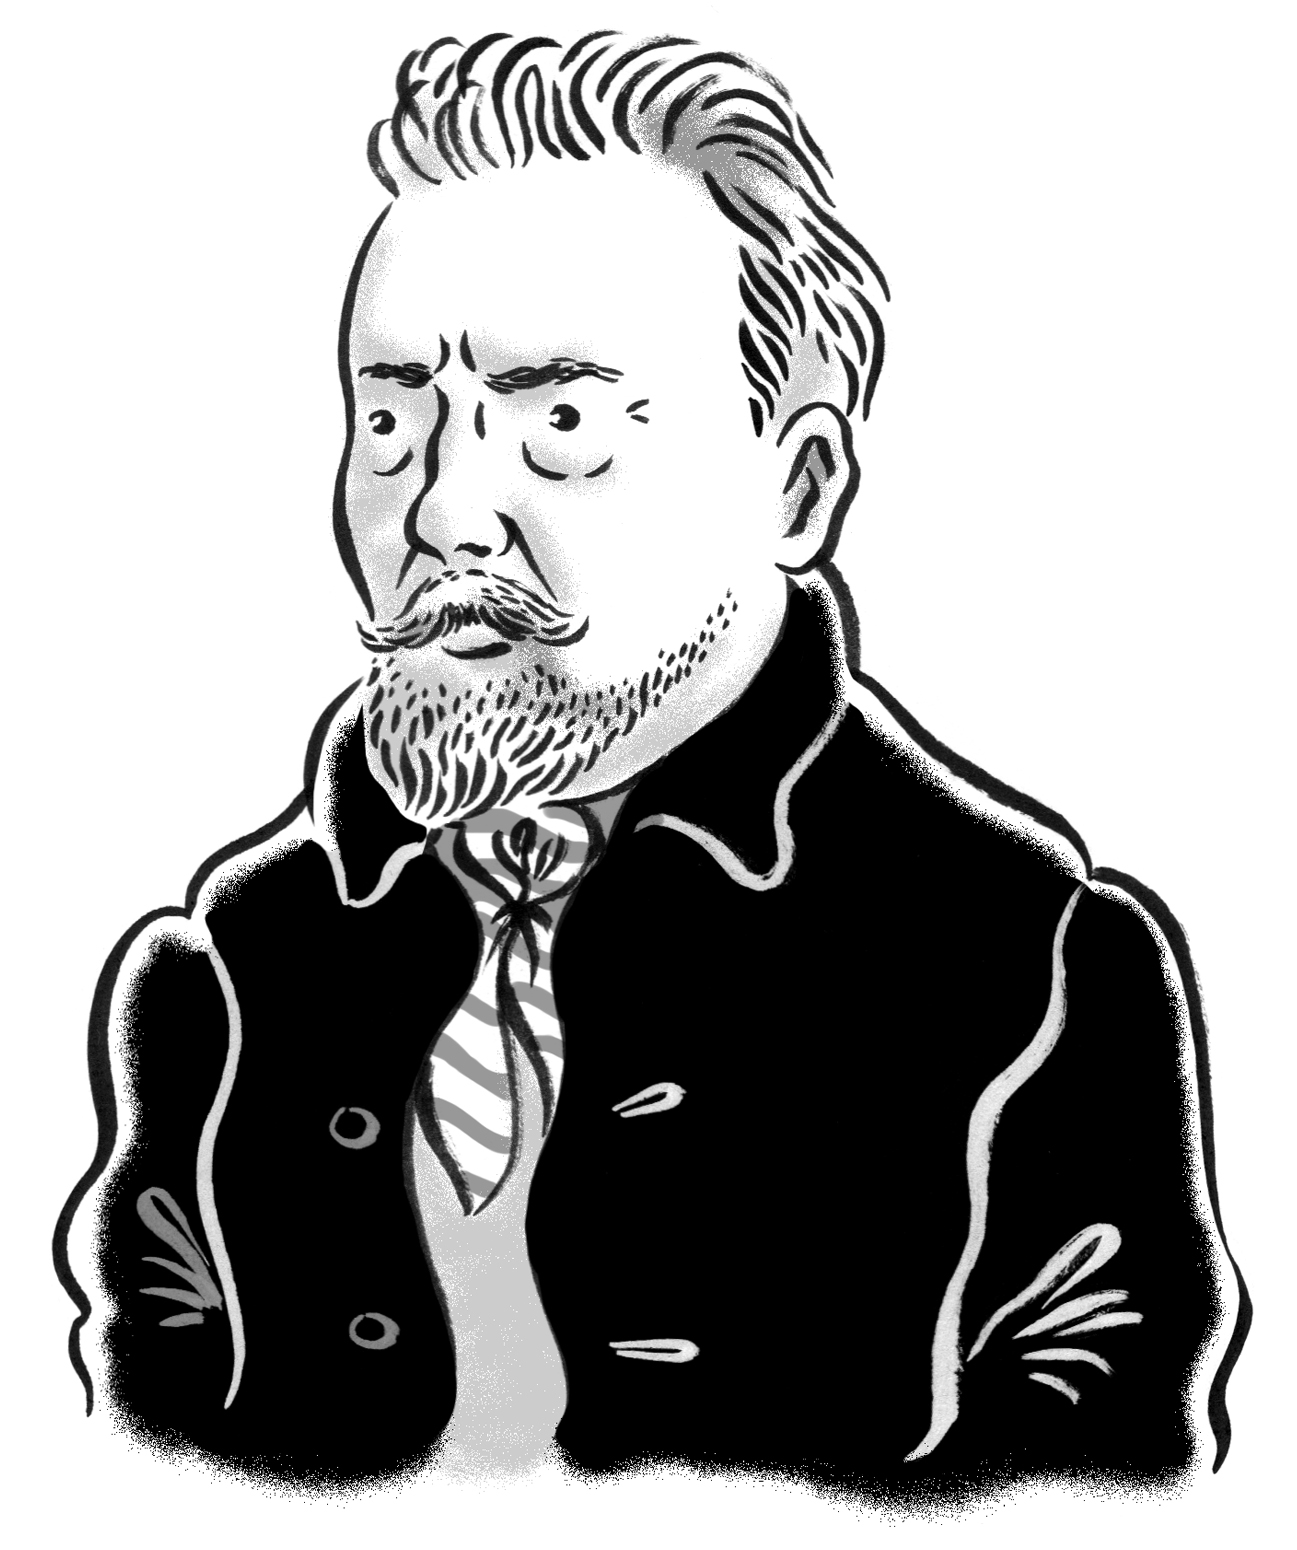
\includegraphics[width=.8in]{./imgs/autor5.jpg}

\noindent{}De origem humilde, Nikolai Leskóv (1831--1895), o mais velho de sete
irmãos, teve vários trabalhos antes de dedicar"-se, nos anos 1860, ao
jornalismo e à literatura. As viagens comerciais que fez pela Rússia ao
trabalhar, em 1857, com um tio de sua esposa, deram"-lhe a oportunidade
de conhecer variados tipos humanos, que foram retratados repetidamente
em suas obras.

O posicionamento independente do escritor o fez colecionar polêmicas
religiosas (chegou a virar tolstoísta) e políticas (ele se indispôs com
conservadores e radicais) nas duas profissões que tinha, que na verdade
coincidiam de certa forma.

Deixou romances, como \emph{A lugar nenhum} (1864), novelas, como
\emph{Lady Macbeth do distrito de Mtzensk} (1865), e muitos contos, como
``O canhoto'' (1881), que, entre realidade e ficção, retratam
camponeses, religiosos, comerciantes, loucos e tratantes, sempre com uma
linguagem saborosa e variegada que usa da sátira e da estrutura dos
contos populares russos.

Parа crianças, publicou na década de 1880 a coletânea \emph{Contos de
Natal} (1886) e textos nas revistas \emph{Palavra sincera} e
\emph{Brinquedinho}, como ``A cabra'' e ``O espantalho''.

O nome de Léskov também se tornou conhecido por um ensaio de Walter
Benjamin sobre o narrador, de 1936, que circulou nos meios acadêmicos e
no qual é acentuado o elemento da oralidade de sua narrativa.

``Bobinho'' (\emph{Duratchók}), conto de Leskóv que mistura, com marcas
de oralidade, duas figuras
emblemáticas da cultura russa --- o \emph{iuródivyi} (misto de louco e
profeta) e o \emph{durák} (personagem dos contos populares) ---, foi
publicado pela primeira vez em 1891 na revista infantil
\emph{Brinquedinho}. Traduzido a partir de:
\textsc{leskóv}, N. \emph{Pólnoie sobránie sotchiniénii.} São Petersburgo:
\emph{Tipografia A. F. Marksa}, 1903, tomo 33.

\pagebreak
\noindent\textbf{ANTON TCHÉKHOV}\medskip

\noindent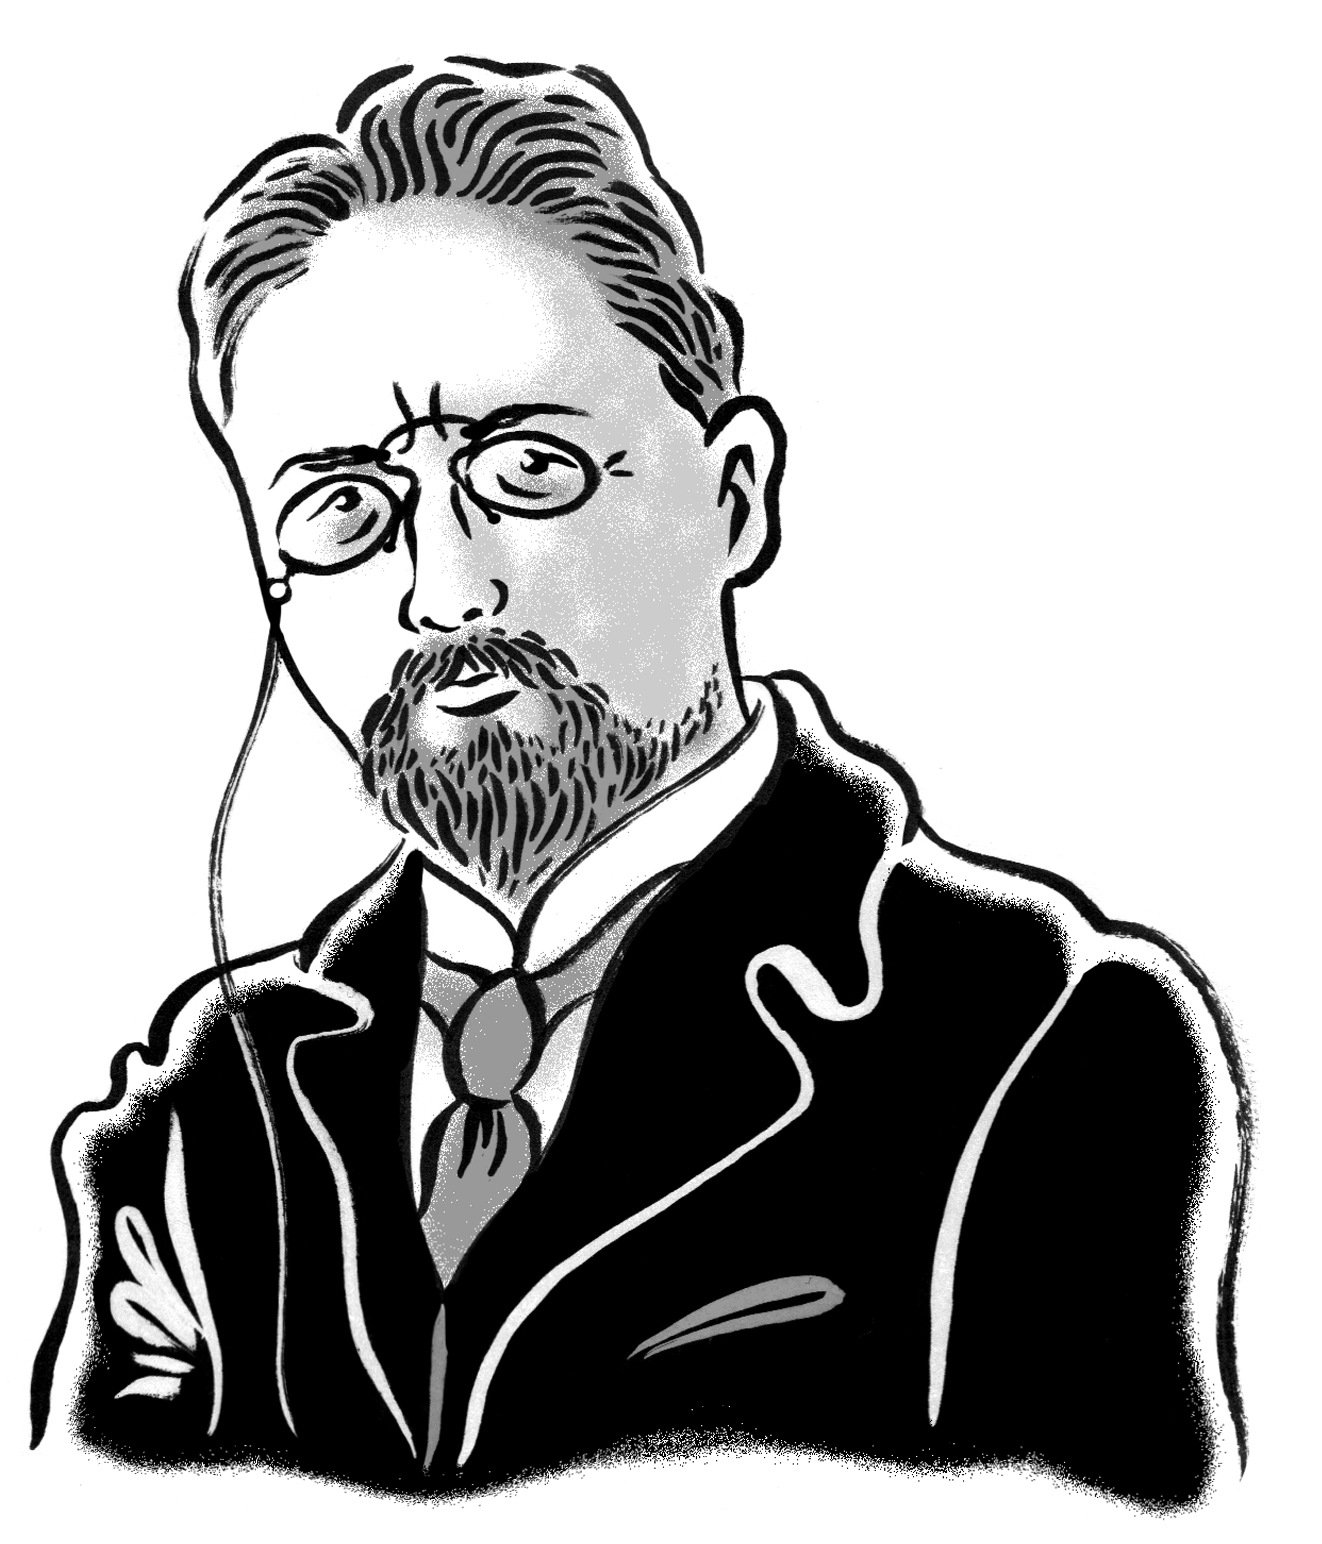
\includegraphics[width=.8in]{./imgs/autor6.jpg}

\noindent{}Anton Tchékhov (1860--1904), escritor e dramaturgo, nasceu numa
cidadezinha chamada Taganrog, no sul da Rússia, e foi o terceiro dos
seis filhos de Pável, dono de uma mercearia, e Evguénia.

Neto de servos, o futuro escritor teve uma infância dura, marcada pela
religião e pela pobreza; seu refúgio eram os livros e o teatro, que o
fascinou desde os 13 anos.

Em 1879, o jovem mudou"-se para Moscou, onde já se encontrava sua
família, que fugira dos credores após a falência do pai. Na cidade
grande, Tchékhov ingressou na faculdade de medicina e continuou
escrevendo pequenas histórias cômicas, publicadas agora em revistas
moscovitas. Produzindo muito e cada vez mais ciente de seu estilo,
transformou"-se num mestre da prosa curta, rompendo com elementos
tradicionais da composição do conto. Muitas de suas obras, como
\emph{Enfermaria nº 6} e ``A dama do cachorrinho'', foram e são
referência para um sem"-número de artistas.

Uma viagem que fizera pelo sul originou a novela \emph{A estepe,}
que, publicada em 1888 na prestigiada revista \emph{Mensageiro do
Norte,} deu"-lhe mais notoriedade. Dois anos depois, o escritor, que
sofria de tuberculose, empreendeu uma difícil e longa viagem a uma
colônia penal na Ilha dе Sacalina, no Extremo Oriente Russo, uma
experiência que teve grande repercussão em sua vida. Ao voltar, passou
os cinco anos seguintes escrevendo um relato sobre a ilha, com
descrições apuradas e denúncias sociais.

Anton Tchékhov também inovou a arte dramática, principalmente com as
peças que criou para o Teatro de Arte de Moscou: \emph{Tio Vânia}
(1899), \emph{As três irmãs} (1901), \emph{O jardim das cerejeiras}
(1904).

Viveu seus últimos anos, entre uma viagem e outra, numa propriedade nos
arredores de Ialta, cuidando da tuberculose, que acabou lhe tirando a
vida precocemente, aos 44 anos. Tchékhov morreu em sua casa, depois de
tomar um copo de champanhe, segundo recordações da atriz Olga Knipper,
sua esposa e amiga.

``Vanka'', assinado com pseudônimo A. Tchekhonte, foi publicado pela
primeira vez no dia 25 de dezembro de 1886 no suplemento ``Contos de
Natal'', do \emph{Jornal de Petersburgo.} Com o autor ainda em vida, o
conto foi incluído no manual escolar \emph{Livro para leitura} (1900) e
traduzido para o francês, o alemão e o dinamarquês. Na história, o órfão
Vanka, de 9 anos, escreve uma carta ao avô para que venha buscá"-lo, uma
carta sem endereço que nunca chegará --- um conto de Natal
antinatalino, como destacaram alguns críticos, com marcas de Andersen,
Dickens e Dostoiévski. ``O fugitivo'' (\emph{Beglets}) saiu em 1887 com
o mesmo pseudônimo e no mesmo jornal. Os dois contos de Tchékhov foram muito
apreciados por Lev Tolstói e se tornaram clássicos da literatura
infantojuvenil russa.
Traduzido a partir de:
\textsc{tchélhov}, A. \emph{Pólnoie sobránie sotchiniénii i pissem v 30 tomákh.}
Moscou: \emph{Naúka,} 1984.

\bigskip
\noindent\textbf{FIÓDOR SOLOGUB}\medskip

\noindent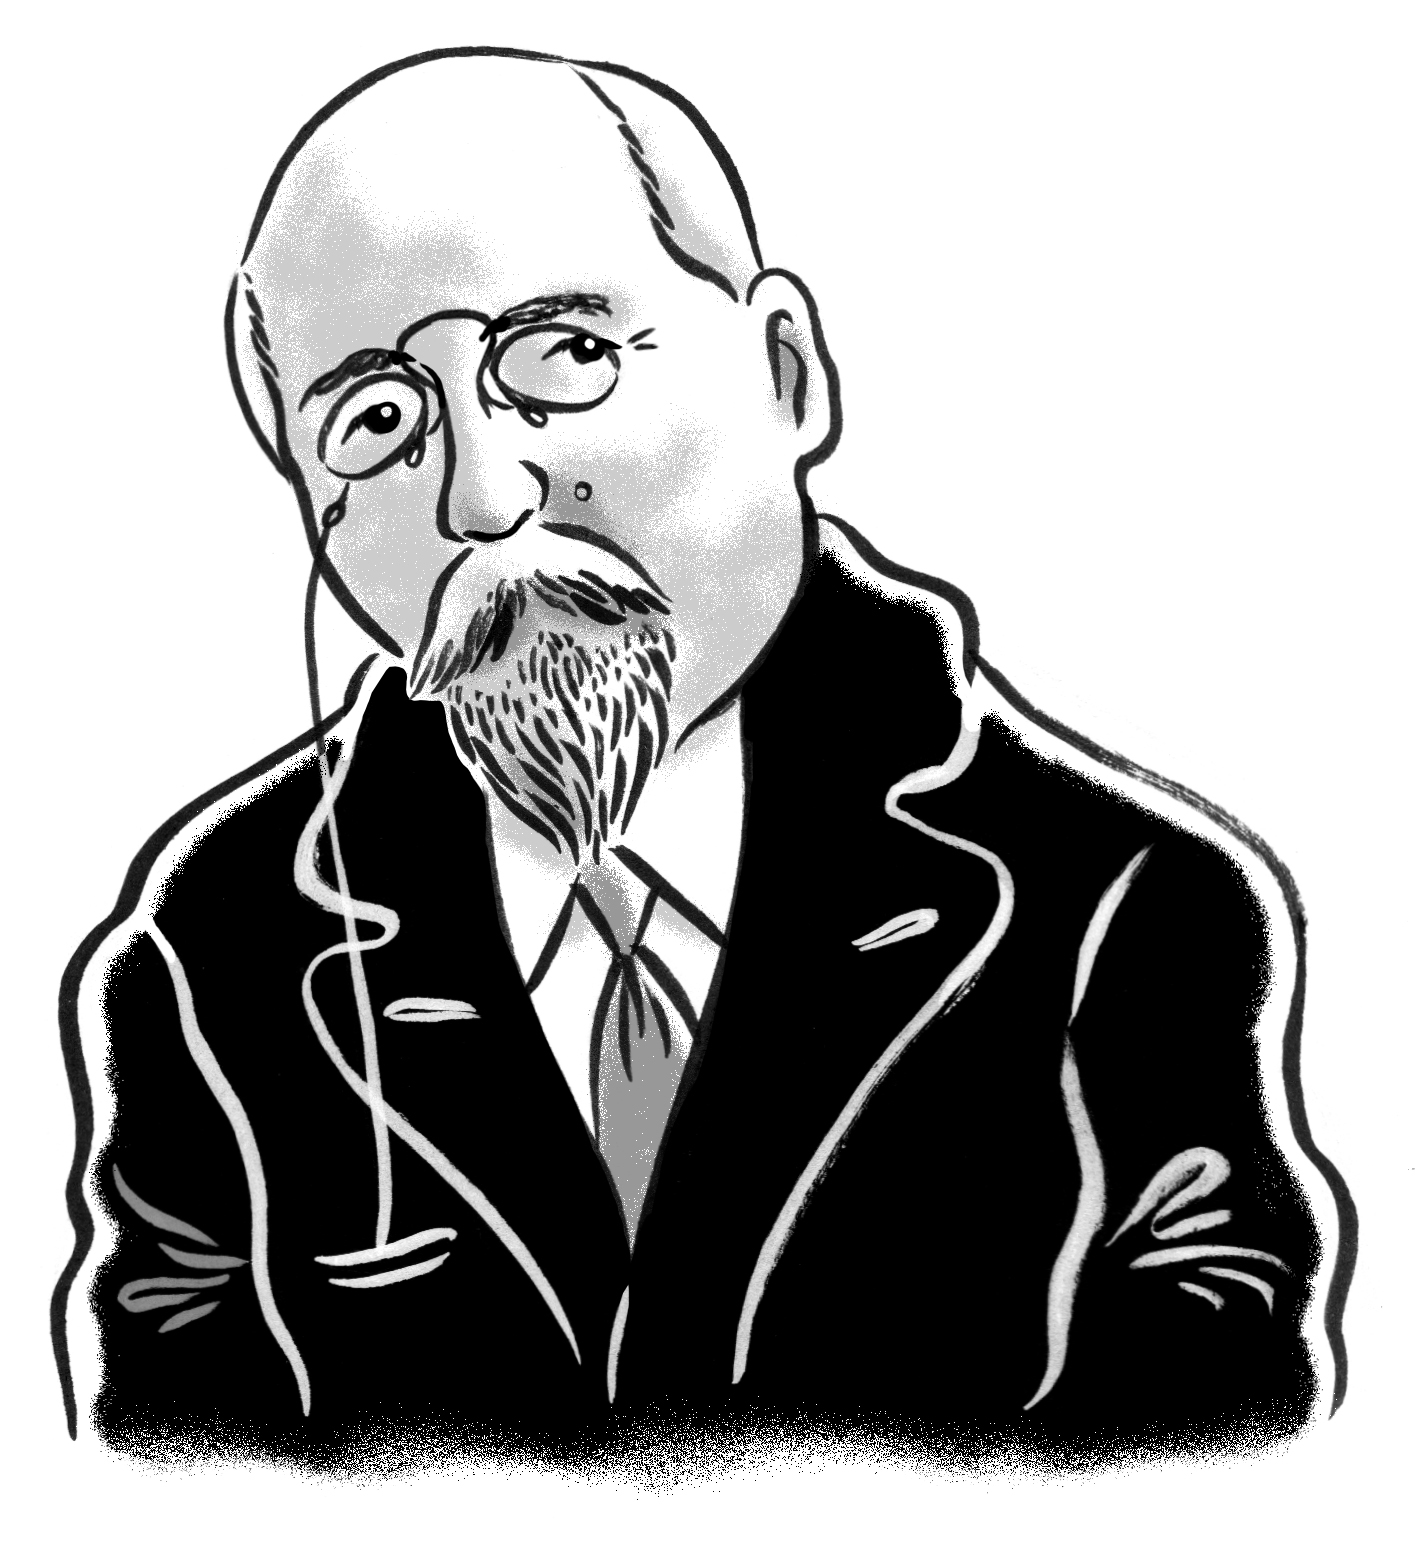
\includegraphics[width=.8in]{./imgs/autor7.jpg}

\noindent{}A figura do poeta, dramaturgo e escritor Fiódor Sologub (1863--1927),
pseudônimo de Fiódor Tetiérnikok, tornou"-se lendária nos meios
literários de sua época. Teciam palavras exultantes sobre sua obra e ao
mesmo tempo o descreviam como um homem de poucas palavras e ausente,
sempre com o pincenê, as pernas cruzadas e os olhos entreabertos.
Sologub foi expoente do simbolismo russo, movimento que floresceu no início do
século \textsc{xx}, produzindo uma renovação poética e estética em diversas áreas
e preparando o advento de novos caminhos para a arte.

Antes do escritor Sologub, vivia o professor Tetiérnikov. Nascido em São
Petersburgo, perdeu o pai, um alfaiate, aos quatro anos de idade. Sua
mãe, severa e religiosa, depois da morte do marido, tornou"-se criada na
casa dos Agápov, uma influente família petersburguesa, onde Fédia, como
o menino era chamado, e Olga, sua irmã mais nova e de quem ele nunca se
separou, passaram a infância e a juventude. Ao concluir o Instituto
Técnico de São Petersburgo, ele trabalhou como professor de matemática e
depois como inspetor escolar até o ano de 1907.

Em 1908, depois da morte de Olga, Sologub se casou com Anastassia
Tchebotariévskaia, tradutora, dramaturga, crítica e sua colaboradora. Em
1921, após inúmeras tentativas frustradas de saírem da Rússia soviética,
Anastassia se jogou da ponte Tutchkóv ao rio Nevá. Fiódor Sologub,
inconformado com a morte da esposa, por muito tempo colocou o prato dela
na mesa de jantar.

A obra de Sologub começou a ser publicada em almanaques na década de
1880, mas foi o ano de 1896 que marcou o início de sua carreira, quando
três de seus livros foram publicados: \emph{Poemas}; \emph{Sombras:
Contos e Versos}; e o romance \emph{Sonhos maus}. Depois teve vasta
carreira literária. Escreveu romances --- como a trilogia \emph{A lenda
criada} (1907--1914) e sua mais afamada obra em
prosa, \emph{O Diabo Mesquinho} (1902) ---, poemas,
ensaios, contos para adultos e crianças e peças de teatro. Suas obras
completas foram lançadas em vida duas vezes; a última, de 1914, tinha 20
volumes.

``A filha do fabricante de caixões'' (\emph{Skazka grobovschíkovoi
dótcheri}), trazendo elementos típicos da prosa simbolista de Sologub,
saiu pela primeira vez em 25 de dezembro de 1915 na revista \emph{Manhã
da Rússia,} em São Petersburgo. Depois o conto, que fala do estranho
amor entre Zoia, cujo pai produzia caixões, e Elnítski, foi incluído na
coletânea \emph{A borboleta cega,} de 1918, publicada pela Editora
Moscovita e considerada uma das melhores do escritor.
Traduzido a partir de:
\textsc{sologub}, F. \emph{Slepaia bábotchka}. \emph{Sotchtiónnye dni}. São
Petersburgo: \emph{Návi Tchári}, 2001.

\bigskip
\noindent\textbf{LÍDIA AVÍLOVA}\medskip

\noindent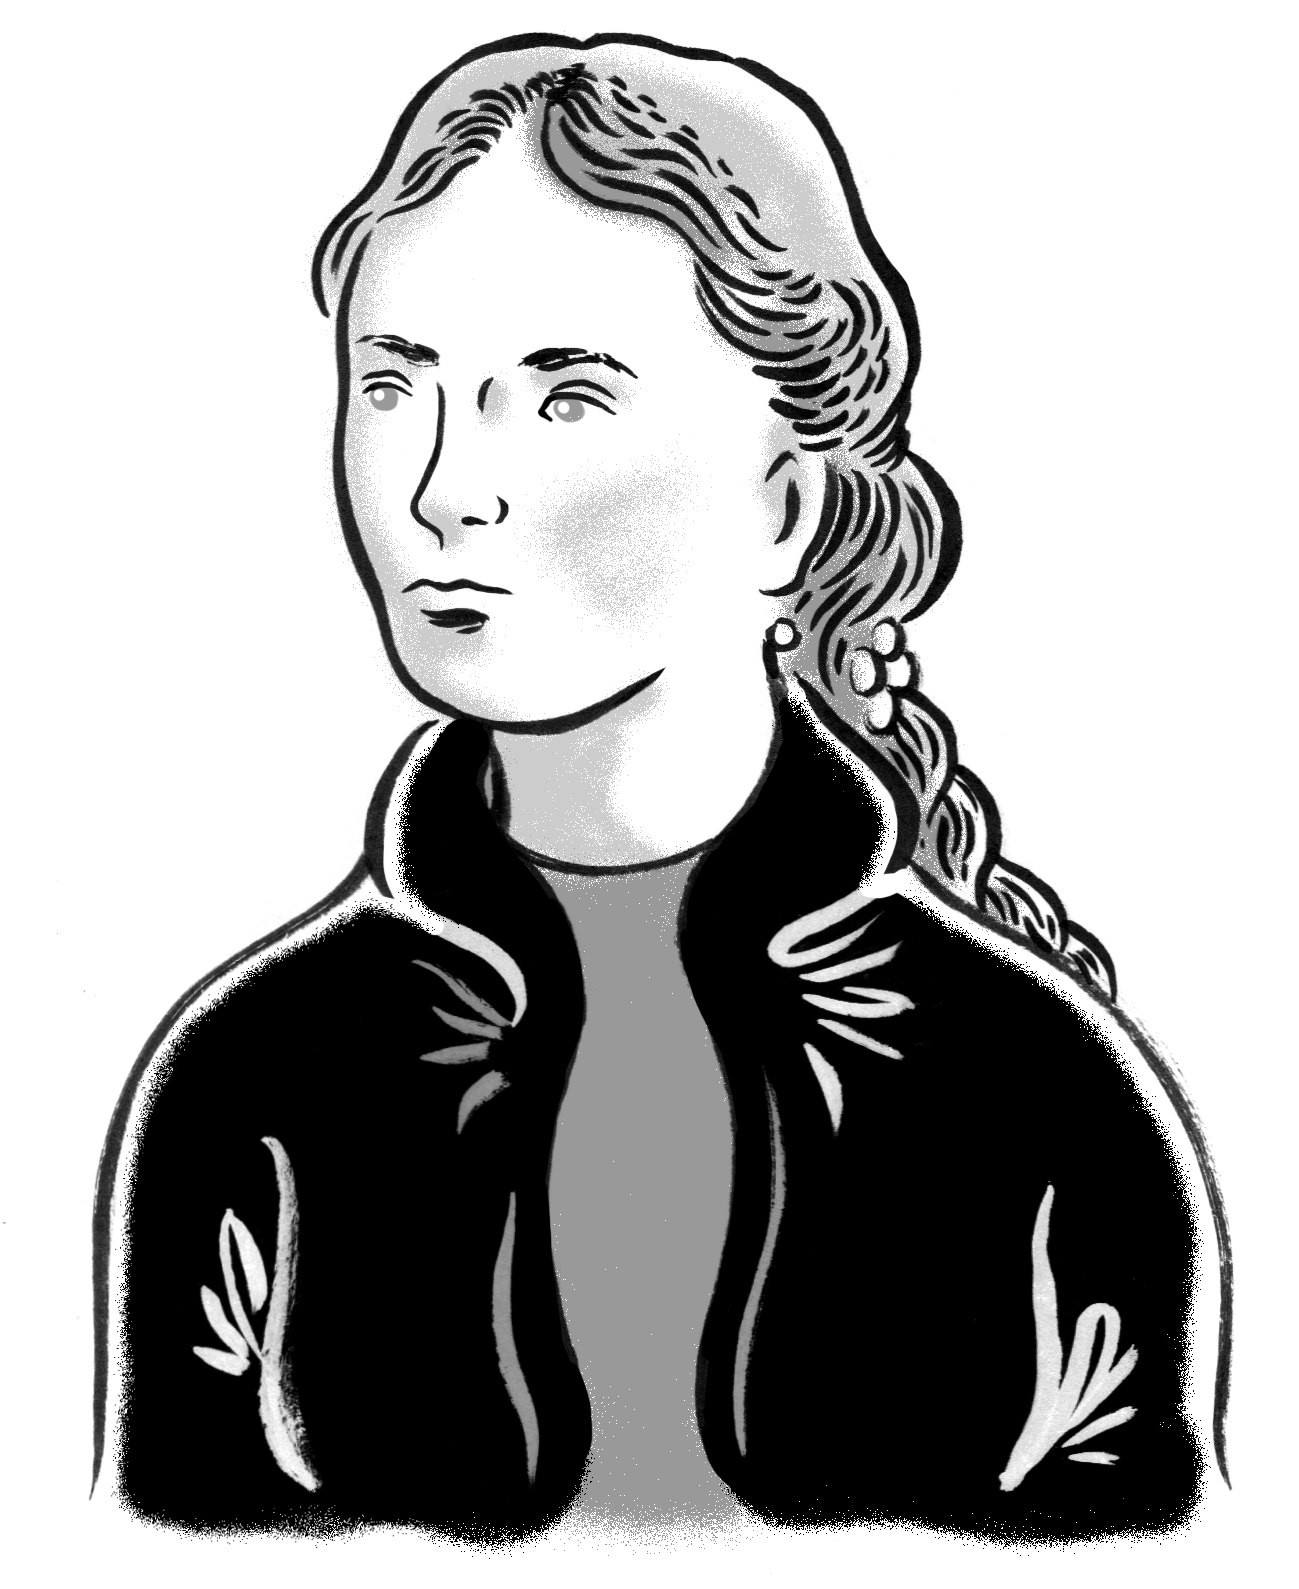
\includegraphics[width=.8in]{./imgs/autor8.jpg}

\noindent{}Oriunda de uma família nobre empobrecida, Lídia Avílova (1864--1943)
desde menina queria ser escritora. Terminou o ginásio em Moscou em 1882
e começou a publicar na década de 1890, colaborando em várias revistas e
edições. Sua primeira coletânea, \emph{O felizardo e outros contos},
saiu em 1896.

Entre seus trabalhos, muitos com temáticas sociais, destacam"-se os
contos (seu gênero favorito) em que sobressai o ponto de vista infantil.
Lídia ``com maestria descortinava o mundo interior da criança, seus
ímpetos e aflições''.\footnote{\scriptsize\textsc{semiónova}, V. G. \emph{Os criadores do
  livro soviético infantil: escritores, poetas, ilustradores}
  (1917--1932) (\emph{Tvórtsy soviétskoi diétskoi knígui: prozaiki,
  poéty, khudójniki}). Moscou: Biblioteca Infantil Еstatal da Rússia,
  2017, p.\,20.}

O nome de Lídia Avílova é geralmente associado ao de Anton Tchékhov, a
quem ela conhecera em 1889 e com quem trocava correspondências, nas
quais o escritor lhe dava conselhos literários. Avílova escreveu a
biografia \emph{A. P. Tchékhov na minha vida}, que acabou se tornando
sua obra mais renomada, embora ela tenha escrito contos e novelas e
tenha sido relativamente conhecida.

Durante a \textsc{urss}, a autora deixou de ser convidada a trabalhar, mas nunca
parou de escrever.

``Primeira mágoa'' (\emph{Piervoie gorie}), de Lídia Avílova,
fez parte de uma coletânea de
mesmo nome publicada em 1919 pela Associação de Editoras de
Escritores, em Moscou, para a Biblioteca Escolar do Povo. O
conto, que descreve o embate do menino Gricha com a realidade de
injustiças sociais ao ver seu cocheiro e amigo ser preso, foi elogiado
por Lev Tolstói, que o integrou à coletânea infantil \emph{Círculo de
leitura} (1906).
Traduzido a partir de:
\textsc{avílova}, L. \emph{Rasskázy, Vospominania.} Moscou: \emph{Soviétskaia
Rossia,} 1984.

\bigskip
\noindent\textbf{ALEKSÁNDR KUPRIN}\medskip

\noindent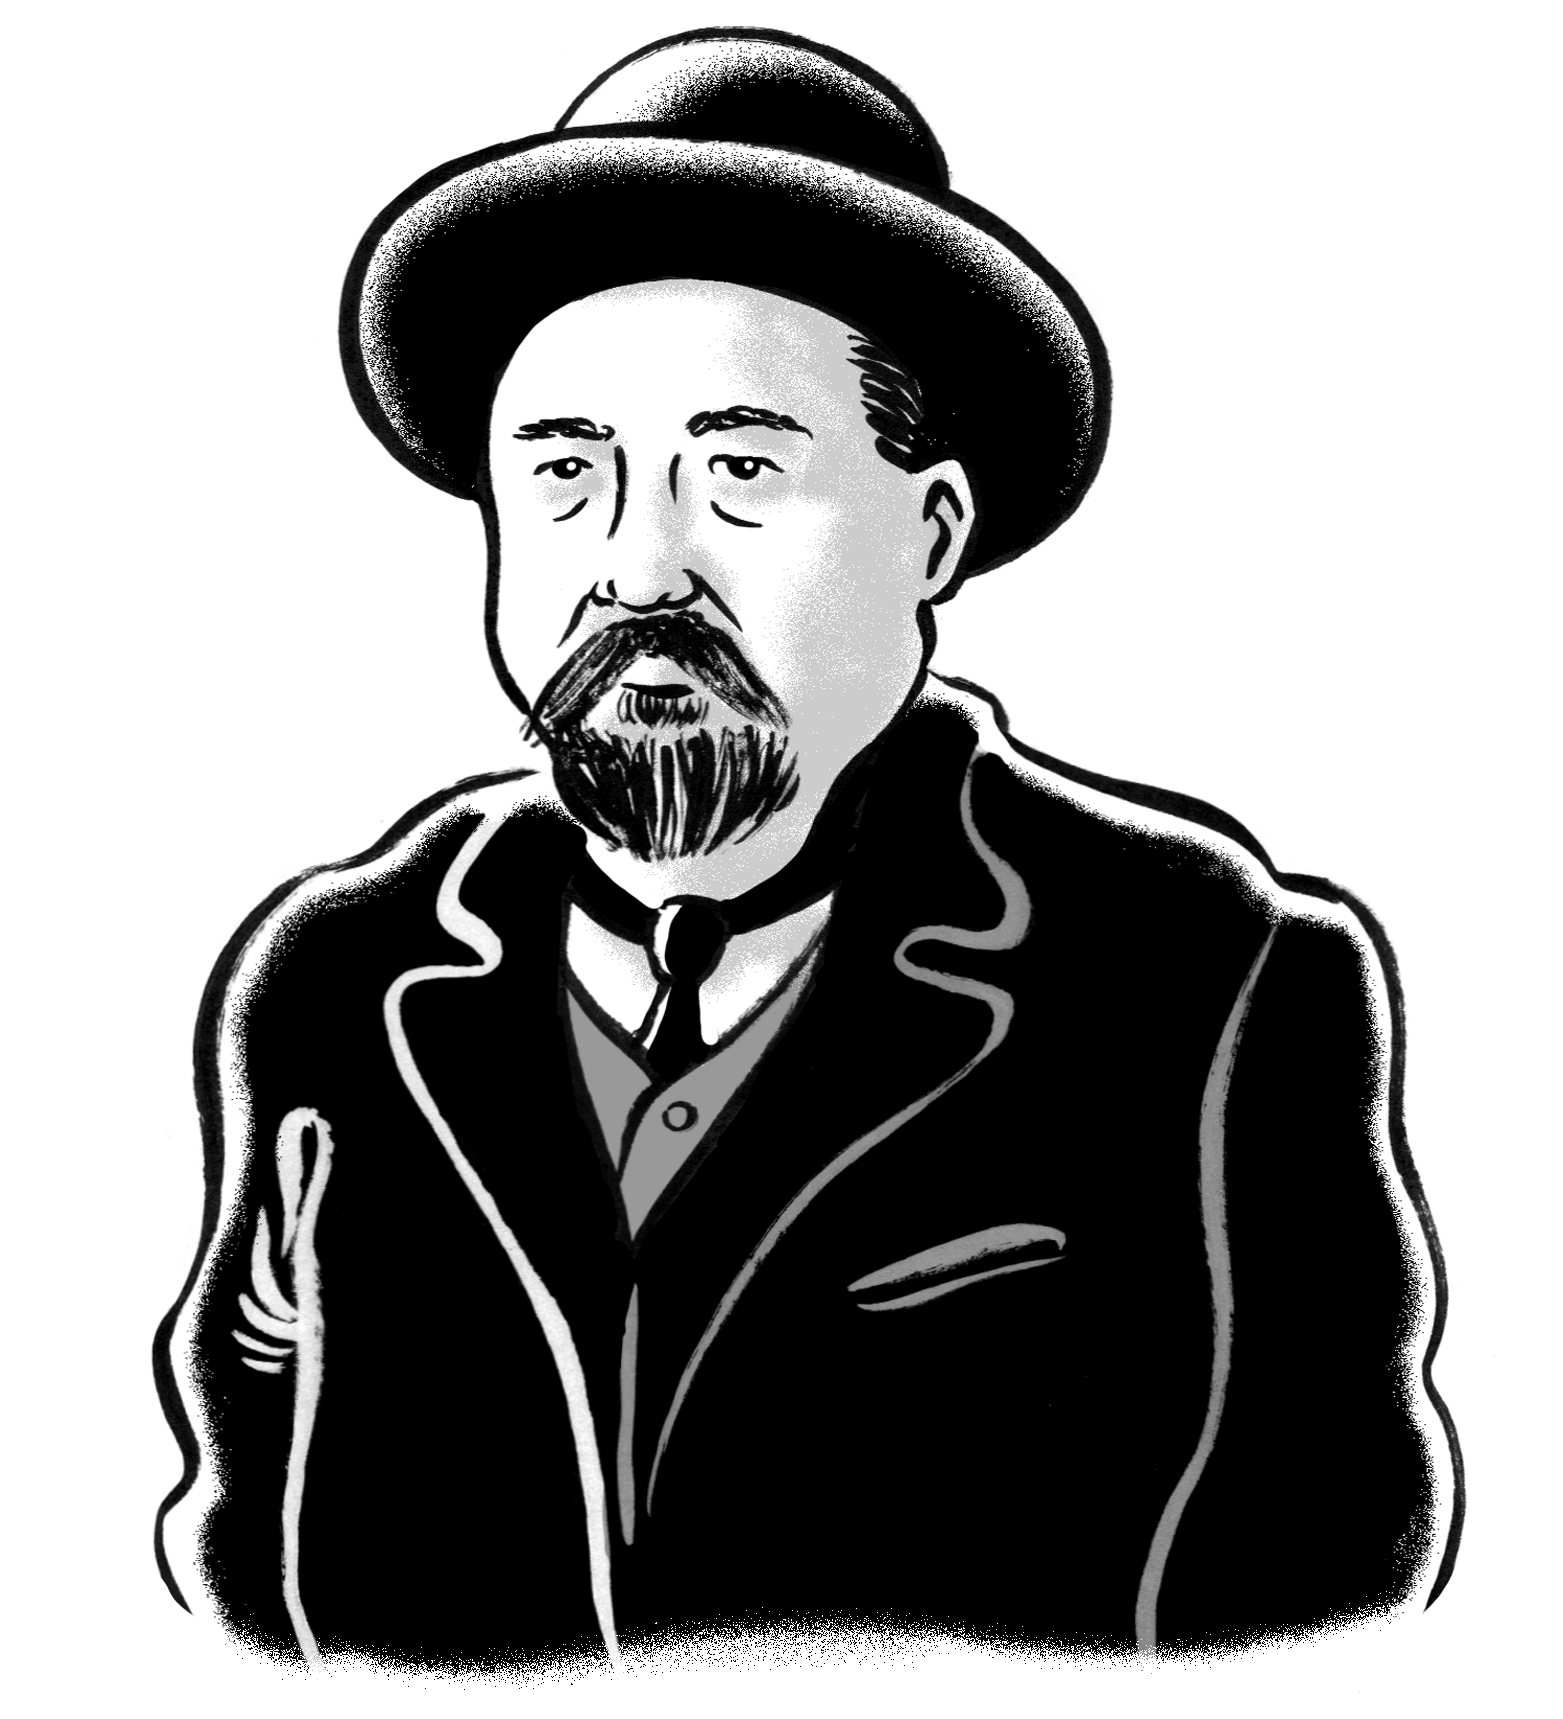
\includegraphics[width=.8in]{./imgs/autor9.jpg}

\noindent{}Aleksándr Kuprin (1870--1938) é lembrado pela personalidade arrojada,
pelo gosto por aventuras, pela vida errante, pelo amor à Rússia, que
conhecia profundamente. Ele nasceu em uma cidadezinha da província de
Penza e com um ano perdeu o pai, Ivan Kuprin, um
funcionário público modesto oriundo da nobreza. Sua mãe, Liubóv Kupriná, de origem tártara, passou por grandes dificuldades e se
viu obrigada a mudar com o filho para Moscou, onde ele estudou em um
colégio militar. Ingressou na Escola de Cadetes de Alexandre em 1888 e,
depois, foi integrado como subtenente ao 46º regimento de infantaria da
guarda imperial е lá ficou até pedir baixa, em 1894. Voltou a alistar"-se
na Primeira Guerra Mundial.

Começou a escrever desde cedo e teve sua primeira obra publicada em
1889: \emph{Estreia derradeira}. No começo da década de 1890, seus
contos começaram a sair em revistas de Petersburgo, onde o autor passou
a morar a partir de 1901. Deixou os quebra"-galhos para trás --- fora de pescador
a ator de circo --- e começou a colaborar em várias revistas como
escritor e volta e meia como jornalista.

Kuprin, simpatizante dos socialistas revolucionários, radicou"-se em
Paris depois da Revolução de Outubro de 1917, regressando à Rússia em
1937.

Com uma prosa franca e realista, Aleksándr Kuprin tratou de diversos
temas, muitos de viés social. Entre seus trabalhos, destacam"-se:
\emph{Moloque} (1896), \emph{O alferes armênio} (1897), \emph{Olessia}
(1898), \emph{O duelo} (1905). Suas histórias infantojuvenis, como
\emph{Doutor milagroso} (1897), \emph{O poodle branco} (1904) е \emph{O
elefante} (1907), são até hoje lidаs pelas crianças russas e estudadas
nas escolas.

O conto ``O elefante'' (\emph{Slon}) saiu pela primeira vez em 1907,
na revista \emph{Vereda}. Já O \emph{poodle branco} (\emph{Biélyi
púdel}), inspirado em fatos reais, em 1904. Kuprin havia ido para o sul
passar um verão e uma trupe aparecera em sua casa: um velho tocador de
realejo, um jovem acrobata chamado Serguei e um \emph{poodle}. Os
saltimbancos passaram a visitá"-lo com frequência e o escritor recebia"-os
com um belo almoço. Foi o acrobata que lhe contou que um dia uma senhora
tentara comprar o cachorro deles. O conto também estabelece diálogo com
``Mumu'' (a volta de Artô para o velho revisita a cena em que Mumu
retorna para Guerássim: os donos estavam dormindo e foram despertados
pelas lambidas dos cachorros, que surgem com um resto de corda no
pescoço). Essa ligação fornece complexidade ao conto de Kuprin, que
ganha contornos mais sombrios: afinal, o que os artistas miseráveis
poderiam esperar do futuro? Não à toa, no fim da história, o velho
estava numa taberna rodeado de homens dormindo, largados no chão, feito mortos.
Traduzido a partir de:
\textsc{kuprin}, A. I. \emph{Ízbrannye sotchiniénia.} Moscou:
\emph{Khudójestvennaia literatura,} 1985.

\bigskip
\noindent\textbf{LÍDIA TCHÁRSKAIA}\medskip

\noindent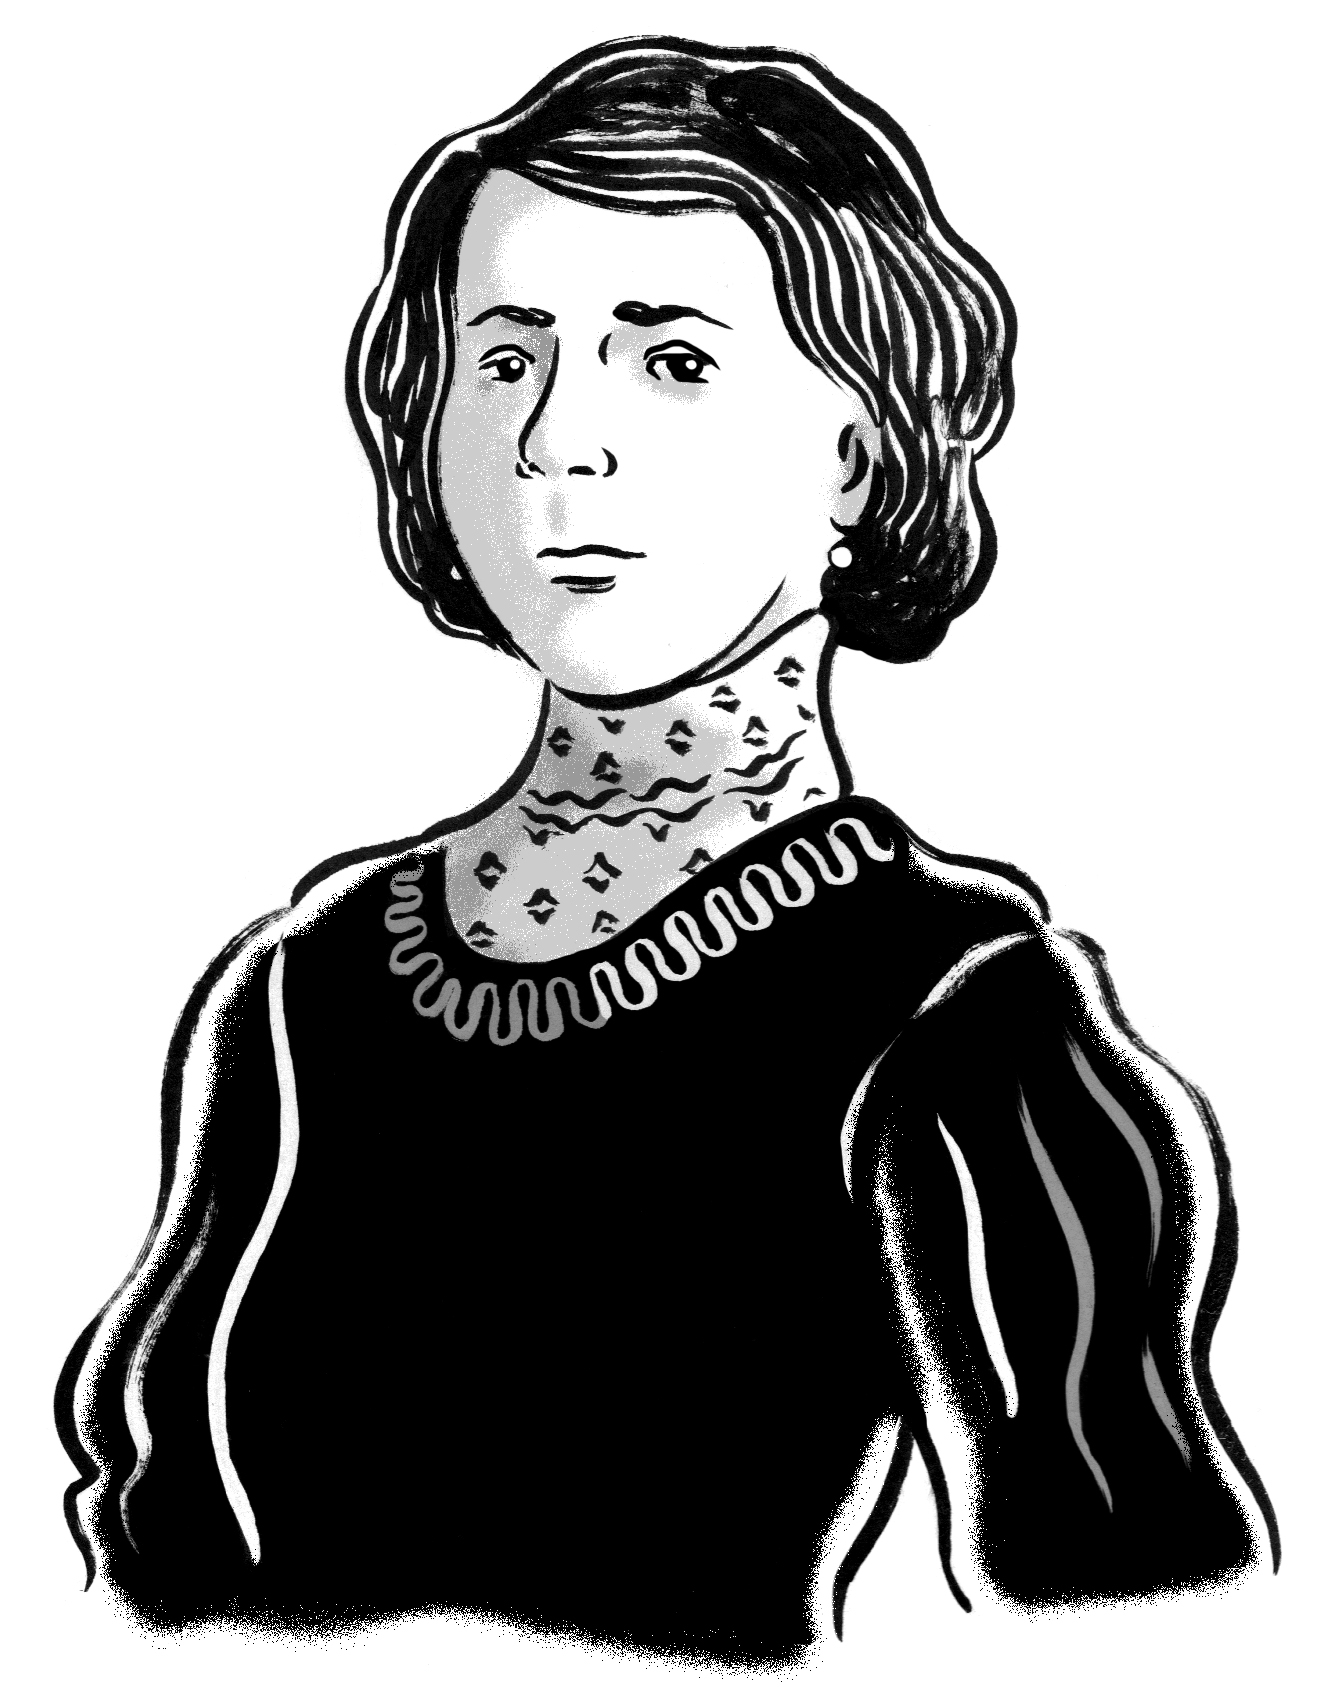
\includegraphics[width=.8in]{./imgs/autor10.jpg}

\noindent{}O nome de Lídia Tchárskaia (pseudônimo de Lídia Tchirilova, 1875--1937),
nascida em Tsárskoie Seló (S. Petersburgo), hoje nem na Rússia é
amplamente conhecido, mas ela foi a autora infantojuvenil mais lida no
início do século \textsc{xx}.

A mãe de Lídia morreu no parto e seu pai era militar. Quando completou
10 anos de idade, por conflitos com a nova família do pai, a menina foi
mandada para o Instituto Pávlovski, um internato para moças, onde ficou
até os 17 anos. Ao sair, ingressou na Escola de Teatro Imperial de São
Petersburgo e, em 1898, tonou"-se parte do corpo de atores do Teatro
Aleksandrínski, fazendo pequenos papéis. Depois de separar"-se do marido,
Lídia começou a escrever para ajudar no sustento do filho e adotou o
pseudônimo Tchárskaia (de \emph{tcháry}, ``feitiço'', ``encanto'').

Com mais de 80 obras publicadas (em geral infantojuvenis), a autora
enveredou por vários gêneros literários: escreveu poemas, contos, contos
maravilhosos, novelas, romances autobiográficos e históricos. Suas
protagonistas femininas --- românticas, sentimentais, positivas e não
raro órfãs (como a própria autora) --- causavam sensação entre russinhas
adolescentes.

\emph{Memórias de uma moça no internato} (1901--1902), sua primeira
novela, foi publicada na revista \emph{Palavra sincera} e fez sucesso
espantoso. Baseada nas lembranças do Instituto Pávlovski, a autora
retrata os conflitos e as expectativas de moças cheias de paixão. As
protagonistas, a pobre ucraniana Liuda Vlássovskaia e a princesa
georgiana Nina Djavakha, deram origem a uma série de livros, que inclui
\emph{A princesa Djavakha} (1903), \emph{Liuda Vlássovskaia} (1904),
\emph{A segunda Nina} (1907), entre outros. A livre e exótica Djavakha,
a quem Marina Tsvetáieva chegou a dedicar um poema na coletânea
\emph{Álbum da tarde} (1910), foi a heroína mais adorada entre as
criações de Tchárskaia.

Com a Revolução de 1917 e a instauração de um novo regime, os livros de
Lídia Tchárskaia, assim como os de outros autores, foram retirados das
bibliotecas e deixaram de ser editados, pois ``elеs eram estranhos à
classe proletária e não correspondiam à nova ideologia'', sendo
considerados por demais sentimentais e ``burgueses''.\footnote{\scriptsize\textsc{hellman}, Ben. \textit{Contos maravilhosos e histórias reais: a história da literatura russa infantil} (\textit{Skazka i byl: Istoria rússkoi diétskoi literatúry}). Moscou: \textit{Nóvoie literatúrnoie obozriénie}, 2016, p.\,179.}
Ela conseguiu driblar a censura por um tempo, usando um pseudônimo, mas,
após ser descoberta, não teve como continuar escrevendo. Foi
despedida do teatro em 1924. Kornei Tchukóvski, Samuel Marchak e Víktor
Chklóvski, representantes de uma nova proposta estética, criticaram"-na
publicamente --- o único que saiu em sua defesa foi Fiódor Sologub,
elogiando a escrita e a popularidade da autora, que acabou morrendo no
ostracismo e na pobreza.

Com o fim da União Soviética, as obras de Tchárskaia voltaram a ser
publicadas na Rússia, embora sem o mesmo frenesi.

``A prova'' (\emph{Ekzámen}), que descreve a ansiedade de uma
menina às vésperas de um exame de geografia, foi retirado da coletânea
\emph{Nuvens azuis}, publicada primeiramente em 1912 em São Petersburgo,
pela Editora V. I. Gubínski. Pela mesma editora saiu ``A mãe''
(\emph{Mat}), retirado da coletânea \emph{Contos da tarde,} sobre o dia
a dia de uma viúva pobre com três filhos pequenos para criar. Ambos os
contos de Tchárskaia têm protagonistas femininas que são descritas em situações
cotidianas, com uma escrita sensível e atenta à psicologia infantil.
Traduzido a partir de: http://charskaya.lit"-info.ru/

\bigskip
\noindent\textbf{SACHA TCHÓRNY}\medskip

\noindent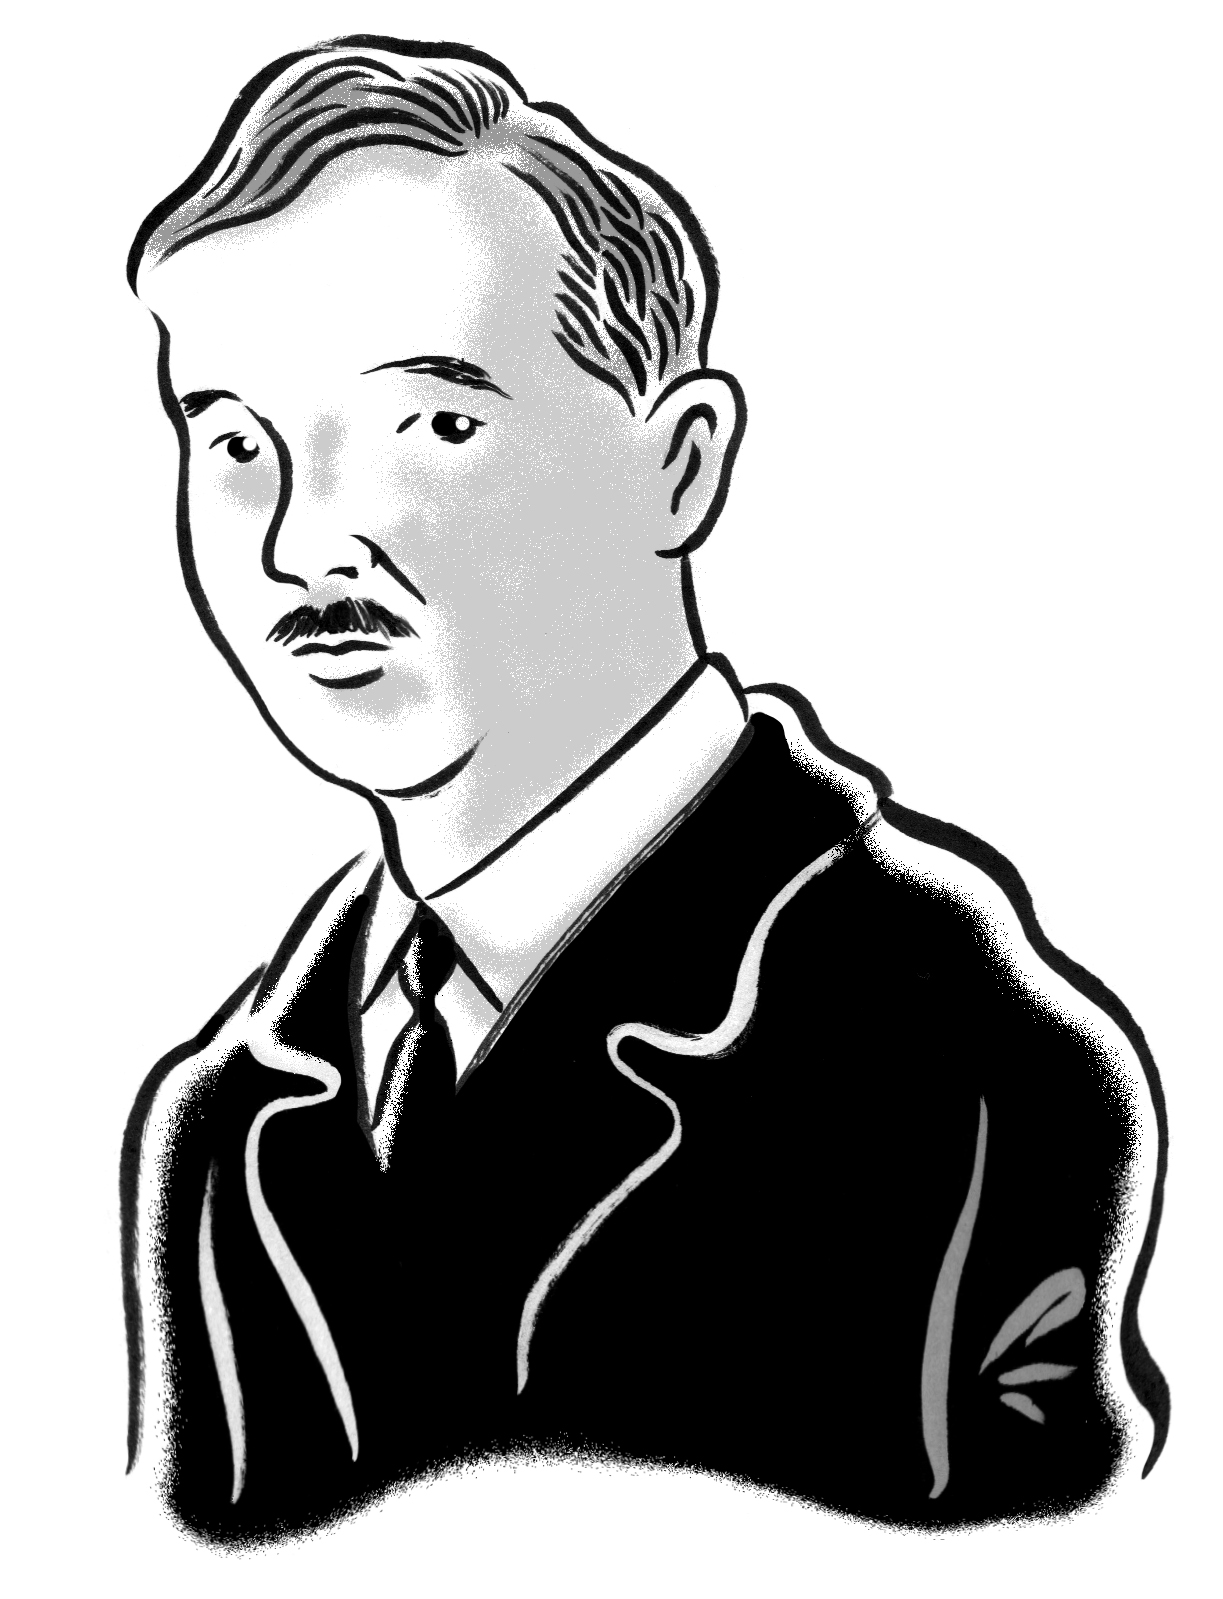
\includegraphics[width=.8in]{./imgs/autor11.jpg}

\noindent{}O poeta e escritor Sacha Tchórny (1880--1932), pseudônimo de Aleksándr
Glíkberg, nasceu numa família judia de Odessa. O \emph{tchórny}
(``preto'' em russo) surgiu porque havia dois filhos chamados Sacha
(apelido de Aleksándr) na família --- um de cabelos pretos, outro de
cabelos loiros.

Sacha Tchórny foi expulso de três ginásios por mau aproveitamento, até
que seus pais pararam de responder às suas cartas e de lhe mandar
dinheiro. Foi um funcionário público de Jitómir que cuidou do menino e
lhe passou o gosto pela poesia.

Tchórny tornou"-se conhecido por seus poemas satíricos, que começou a
publicar em 1901. Já morando em São Petersburgo, passou a colaborar em
várias revistas, e seus versos cômicos eram esperados ansiosamente pelos
leitores, que os sabiam de cor. Esses textos críticos tornaram o autor
alvo da censura e ele se viu obrigado a ir para a Europa, de onde voltou
em 1908. Agora um poeta renomado, virou colaborador da revista
\emph{Satirikon.}

A partir de 1911, para a surpresa dos admiradores de sua veia irônica, o
escritor ingressou na literatura infantil. Ele fez tanto sucesso como
poeta para os pequenos quanto para os grandes. Ao universo infantil
trouxe humor, ritmo poético е uma linguagem própria da criança, dando
sinais da nova fase da literatura russa para a infância que se
consolidará alguns anos depois.

Em 1918, depois de voltar do \emph{front} da Primeira Guerra Mundial,
Tchórny emigrou para a Europa, onde continuou escrevendo textos para
crianças. Tornou"-se colaborador da revista \emph{Varinha verde} e
publicou muitos livros infantojuvenis, tais como a antologia poética
\emph{A ilha infantil} (1921) e \emph{O diário do fox Mikki}
(1927), uma história contada do ponto de vista de um cachorro
parisiense.

O conto ``A pedrinha vermelha'' (\emph{Krásnyi kámechek}) foi impresso
pela primeira vez em 1912 na coletânea \emph{Livrinho azul,} da qual
participou também Maksim Górki. Mas quem brilhou dessa vez foi Tchórny,
com uma história cheia de fantasia e graça em que o menino Jórjik,
passeando pela floresta, recebe de uma velha uma pedrinha mágica. Ao
ser colocada no ouvido, ela lhe dá o poder de conversar com os animais.
Traduzido a partir de:
\textsc{tchórny}, S. \emph{Dniévnik Foksa Mikki: Póvest, skaska, stikhi}. Moscou:
\emph{Makhaon}, 2015.

\pagebreak
\noindent\textbf{DANIIL KHARMS}\medskip

\noindent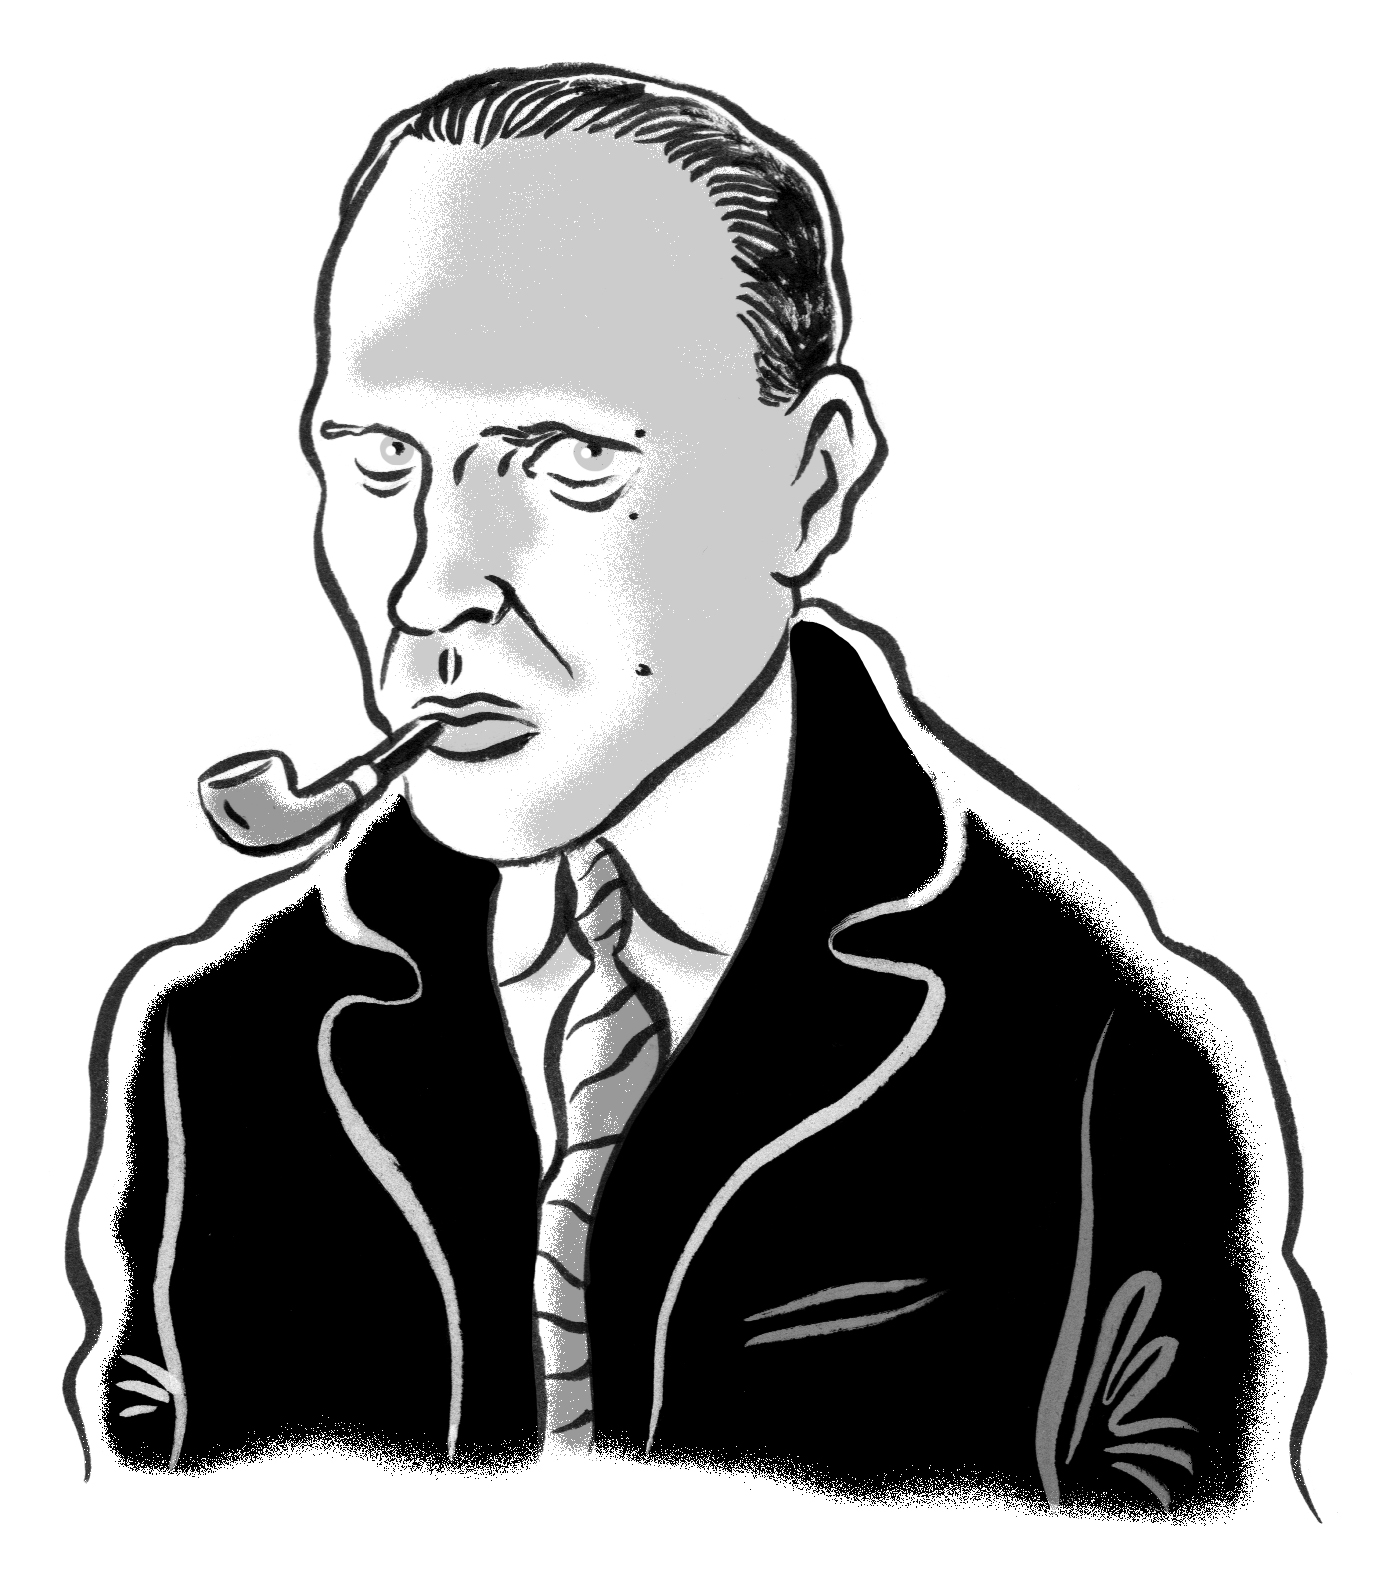
\includegraphics[width=.8in]{./imgs/autor12.jpg}

\noindent{}Daniil Kharms (1905--1942), pseudônimo de Daniil Iuvatchóv, foi um
escritor, poeta e dramaturgo nascido em São Petersburgo. Um dos
precursores do teatro do absurdo com a peça \emph{Elizaveta Bam} (1928),
que criou para a noite de estreia da \textsc{oberiu} (Associação para uma arte
real), ele é hoje equiparado a escritores como Franz Kafka, Eugène
Ionesco e Samuel Beckett.

O excêntrico Kharms (de \emph{harm}, ``mal'' em inglês), na década de
1920, vestia"-se com itens da indumentária de Sherlock Holmes (seu herói
favorito), participava ativamente de círculos de vanguarda, praticava
jiu"-jítsu, ioga e xadrez, e se interessava pelo ocultismo e pela cabala.

1928 foi o ano em que nasceu a \textsc{oberiu}, de que participaram também poetas
como Aleksándr Vvediénski e Nikolai Zabolótski, e o ano em que nasceu o
escritor para criança Kharms --- ele passou a colaborar nas revistas
\emph{Ouriço} (\emph{Ioj}) e \emph{Pintassilgo} (\emph{Tchij}) e deixou
vários livros infantis (seus trabalhos para adultos não eram
publicados), tais como: \emph{Um fusível travesso} (1928); \emph{Teatro}
(1928); \emph{Ivan Iványtch, o samovar} (1929); \emph{Sobre como uma
velhinha comprou tinta para escrever} (1929); \emph{Em primeiro lugar e
em segundo lugar} (1929).

Ele enveredou para a literatura infantil para conseguir um ganha"-pão,
mas tinha um dom natural para criar histórias lúdicas, cheias de humor,
com jogos engenhosos de palavra e ritmo musical. Além disso, esse
trabalho lhe permitiu fazer apresentações, pois a revista patrocinava
idas de escritores a escolas e jardins de infância. Daniil aparecia
muito sério, em toda a sua estranheza (era muito alto e muito magro) e,
depois de alguns truques de mágica, lia seus contos e poemas, e os
pequenos o ouviam admirados. O curioso é que ele próprio escreveu mais
de uma vez que não suportava crianças\ldots{} Mas quem poderia afirmar quando
Kharms falava a sério ou não?

Na década de 1930, depois da dissolução da \textsc{oberiu} e de sua primeira
prisão (mais pela literatura infantil do que por suas apresentações
artísticas escandalosas), a obra do escritor para adultos ganhou linhas
mais minimalistas e filosóficas. Distante da realidade soviética, muito
isolado e quase sem condições de sobreviver, produziu principalmente
trabalhos em prosa, como a série \emph{Causos} (1933--39) e \emph{A
velha} (1939), sua única novela, obras"-primas que só chegaram ao
conhecimento do grande público depois de 1990. Sua segunda prisão, por
``atividades antissoviéticas'' (condenação genérica da época), ocorreu
em 1941; ele foi transferido para uma ala psiquiátrica e morreu de fome
no ano seguinte.

\emph{Sobre como Kolka Pánkin viajou para o Brasil e sobre como Pietka
Erchóv não acreditou em nada} (\emph{O tom, kak Kolka Pánkin letal v
Braziliu, a Pietka Erschóv nitchego ne viéril}) saiu na revista
\emph{Ouriço} (nº2), em 1928, e depois, no mesmo ano, em forma de livro,
com tiragem de 20000 exemplares e ilustrações de Evguenia Evenbakh, pela
Editora Estatal. A viagem de dois meninos para o Brasil é um exemplo
magistral do \emph{nonsense} infantil, dialogando com autores como
Edward Lear e Samuel Marchak, a quem Kharms considerava um mestre.
Traduzido a partir de:
\textsc{kharms}, D. \emph{Pólnoie sobránie sotchiniénie}, em três volumes.
Organização Valéri Sájin. São Petersburgo: \emph{Ázbuka}, 2011.

\bigskip

\noindent\textsc{Daniela Mountian}

\chapter{Sobre os colaboradores}


\noindent\textbf{Daniela Mountian}, criadora da Kalinka, atualmente faz pós"-doutorado sobre literatura infantil russa e brasileira (\textsc{usp/fapesp}).

\noindent\textbf{Fido Nesti} é ilustrador e cartunista com trabalhos na \textit{Folha de S.Paulo} e \textit{The New Yorker}. Entre suas várias publicações, consta \textit{1984}, de George Orwell, que ilustrou e adaptou.

\noindent\textbf{Irineu Franco Perpetuo} é tradutor, jornalista e crítico de música. Entre suas muitas traduções, consta \textit{Vida e destino}, de Vassíli Grossman.

\noindent\textbf{Moissei Mountian}, nascido na \textsc{urss}, é tradutor e criador da Kalinka. Traduziu muitos livros russos, tal como \textit{O Diabo Mesquinho}, de Fiódor Sologub.

\noindent\textbf{Nanami Sato}, mestre e doutora na área de didática (\textsc{usp}), foi professora de português na Faculdade Cásper Líbero (Jornalismo).

\noindent\textbf{Paulo Henrique Pompermaier} é formado em Jornalismo pela Faculdade Cásper Líbero e é editor"-assistente da Editora Hedra.

\noindent\textbf{Tatiana Larkina}, nascida em Moscou, é tradutora e professora de russo com mestrado na \textsc{usp}. Entre suas traduções, consta \textit{O Silvano}, de Anton Tchékhov.

\endgroup

\pagebreak
\pagestyle{empty}
\movetooddpage
\pagestyle{empty}

\scriptsize{
\noindent{}CATÁLOGO DA EDITORA KALINKA\\[5pt]

\noindent{}O Diabo Mesquinho\\
FIÓDOR SOLOGUB
\medskip

\noindent{}Encontros com Liz e outras histórias\\(Coleção Contos russos modernos, 1900-1930)\\
LEONID DOBÝTCHIN
\medskip

\noindent{}“Os sonhos teus vão acabar contigo”: prosa, poesia, teatro\\(Coleção Contos russos modernos, 1900-1930)\\
DANIIL KHARMS
\medskip

\noindent{}Luminescência: antologia poética\\
VIATCHESLÁV KUPRIYÁNOV
\medskip

\noindent{}Luminescência: desdobramentos\\
VIATCHESLÁV KUPRIYÁNOV
\medskip

\noindent{}Poesia russa: seleta bilíngue
\medskip

\noindent{}Tarakã, o bigodudo (Ars et Vita e Kalinka)\\
KORNEI TCHUKÓVSKI
\medskip

\noindent{}Parque Cultural\\
SERGUEI DOVLÁTOV
\medskip

\noindent{}Salmo\\
FRIEDRICH GORENSTEIN
\medskip

\noindent{}O ofício\\
SERGUEI DOVLÁTOV
\medskip

\noindent{}O elefante (Coleção Mir)\\
ALEKSÁNDR KUPRIN
\medskip

\noindent{}A velha (Coleção Mir)\\
DANIIL KHARMS 
\medskip

\noindent{}Bobók \& ‘Meia carta’ de um sujeito (Coleção Mir)\\
FIÓDOR DOSTOIÉVSKI
\medskip

\noindent{}Aulas de literatura russa: de Púchkin a Gorenstein \\
AURORA FORNONI BERNARDINI
\medskip

\noindent{}O compromisso\\
SERGUEI DOVLÁTOV
\medskip

\noindent{}A Cidade Ene (Coleção Contos russos modernos, 1900-1930)\\
LEONID DOBÝTCHIN
\medskip

\noindent{}O diabo (Coleção Mir)\\
MARINA TSVETÁIEVA
\medskip

\noindent{}A infância de Nikita (Coleção Bella)\\
ALEKSEI TOLSTÓI
\medskip

\noindent{}Contos russos juvenis (Coleção Bella)\\
DANIELA MOUNTIAN (ORG.)

\pagebreak
\thispagestyle{empty}
\movetooddpage
\thispagestyle{empty}

\begingroup\footnotesize

\vspace*{\fill}
\begin{flushright}
CONTOS RUSSOS JUVENIS\\[6pt]
Copyright © Kalinka, 2021\\[6pt]
Prefácio © Daniela Mountian\\[6pt]
Tradução © Irineu Franco Perpetuo\\[6pt]
Tradução © Moissei Mountian\\[6pt]
Tradução © Tatiana Larkina\\[20pt]

primeira edição, 2021\\[20pt]

Esta publicação está de acordo com a reforma ortográfica.\\[6pt]

As notas de rodapé são da tradução com colaboração da edição, com exceção das observações dos próprios autores, assinaladas pontualmente.\\[6pt]
\end{flushright}
\vspace*{\fill}

\vfill


\begin{flushright}
\textbf{EDIÇÃO}\\
\textbf{Editora Kalinka}\\
Avenida Angélica, 501 cj. 306\\
01227-900 São Paulo-SP Tel.11 2579-6290\\
www.kalinka.com.br\\[10pt]

\textbf{PRODUÇÃO EXECUTIVA}\\
\textbf{Editora Hedra}\\
Rua Fradique Coutinho, 1139 Vila Madalena\\
05416-011 São Paulo-SP Tel.11 3097-8304\\
www.hedra.com.br
\end{flushright}

\endgroup

\pagebreak
\mbox{}\vfill\small\thispagestyle{empty}
\begin{center}
		\begin{minipage}{.7\textwidth}
		\centering\tiny\noindent{}Este livro foi impresso pela primeira vez no ano de 2021. \begin{center}\normalsize\adforn{64}\end{center}
		\end{minipage}
\end{center}